\documentclass[openright]{template/uva-bachelor-thesis}
\usepackage{graphicx}
\usepackage{url}
\usepackage{enumitem}
\usepackage{multicol}
\usepackage{csquotes}
\usepackage[margin=1cm,format=hang]{caption}
\usepackage{subcaption}	
\usepackage{pdflscape}
\usepackage{float}
\usepackage{tocbibind}


\usepackage{hyperref}
\usepackage{cleveref}

\usepackage[style=ieee,backend=bibtex]{biblatex}
\addbibresource{cite.bib}

% Title Page
\title{A model for \\experiment setups on\\ FPGA development boards}
\author{Matthijs Bos}
\supervisors{Toto van Inge (UvA), Taco Walstra (UvA), Edwin Steffens (UvA)}
\signedby{n.a.}


\begin{document} 

\maketitle

\begin{abstract}
TODO
\end{abstract}

\tableofcontents

\chapter{Introduction}
\label{chapterintroduction}
% nog niet helemaal logisch
The use of field-programmable gate arrays (FPGA) has increased a lot in the past years. FPGAs have been successfully applied in many industries as well as in academic research. Manufacturers have put a great effort in further developing the capabilities of FPGAs, resulting in an increase in performance and size, as well as a decrease in power consumption and unit cost. Due to their high cost, FPGAs used to be unsuitable for application in classroom teaching. The developments of the past years however, put FPGAs within the reach of academic education. Nowadays, a full-featured FPGA development board can be acquired for under \$150. 

Computer architecture and organization is considered an important subject in the computer science program taught at the University of Amsterdam (UvA). The subject is taught to freshmen as an eight week course in an early stage of their curriculum. The subject's body of knowledge ranges from a low level understanding of a computer's central processing unit's (CPU) inner workings, design and surrounding systems to a more abstract view of the CPU that considers its instruction set from a software point of view.

% SIM-PL welof niet noemen?
% Minder vanuit UvA, Meer vanuit Henessy and Patterson
% dieper ingaan op experimenten?
% meer focus op high-level, minder op digital design
The UvA's course contents are based on the widely adopted works of Hennessy and Patterson, supported by a number of lab experiments. These lab experiments allow students to reinforce their theoretical understanding of the course's subject matter by interacting with a number of virtual computer architectures in a simulator environment. In the process of modernizing the computer architecture and organization course, the instructors sense the need for a more hand-on experience in which students are capable of interacting with physical devices. This physical view of a computer architecture may aid in a student's understanding of the subject matter.

Hardware design is not part of the computer science curriculum.

Using FPGAs to experiment with (variations of) live computer architecture implementations to perform qualitative experiments instead of doing (partial) actual implementation. HDL programming is not a part of the curriculum.

FPGAs allow for a computer architecture design to be taken out of the virtual environment of a simulator and be implemented in a physical device. As such, they may provide a solution in achieving the goals of the UvA's computer architecture and organization course instructors. The technical capabilities of FPGAs combined with the decreased cost of FPGA development boards makes their adoption in the course a viable option. 

Utilizing FPGAs however, is a complex task that requires a specific set of skills, including digital design, hardware definition language (HDL) programming and familiarity with specialized development tools. Their complexity and the set of skills required raises problems in the application of FPGAs in an eight week introductory level computer architecture and organization course. Each of these skills may deserve a course on their own and are mostly beyond the scope of the UvA's undergraduate computer science curriculum. 

This thesis presents a generic solution that allows for students to utilize FPGAs in their lab experiments without the requirement of these more advanced skills. Experiments are performed using a Digilent Nexys 4 FPGA board, connected to a PC. An implementation is provided and validated through a number of experiments in which multiple variants of Hennessy and Patterson's MIPS computer architecture are running on an FPGA. The scope of this thesis is limited to a technical solution and does not evaluate the didactic effects of a hands-on approach in the teaching of these subjects.

\section{Related work}
Traditionally, computer architecture and organization lab experiments make use of virtual environments in the form of simulators. Many of these simulators exist, each with a different scope and level of detail. In particular, computer architecture simulators are used, which simulate the behaviour of a microprocessor. Some simulators such as the SPIM MIPS simulator \cite{spim} only feature a simulation of the instruction set and register state, while others provide a cycle accurate simulation of a specific microprocessor implementation, allowing for accurate evaluation of performance metrics. For their computer architecture and organization lab experiments, the UvA's course instructors makes use of the SIM-PL simulation environment \cite{simpl}, which was developed at the UvA. The SIM-PL simulator allows for a cycle-accurate simulation of the execution of a particular computer architecture that is implemented using digital design primitives through a graphical interface.

% FPGAs have been used in the courses of other universities' curricula before, including the teachings of the subject of computer architecture and organization. 

%Masters or late bachelor curriculum
Jansen and Dusch \cite{jansen2014every} present a method that teaches electrical engineering master students to apply their available knowledge of HDL programming and digital electronics in order to implement and verify different parts of a microprocessor in VHDL. At the end of the course, students combine their previous results into a working microprocessor in order to produce a working system which is programmed onto a FPGA. After achieving a working setup on a FPGA, students are required to test their work by writing and running a simple c program. The course instructors provide the tools and a simple operating system in order to compile and run the student programs. 

In the works of Cifredo-Ch\'acon et al. \cite{cifredo2015computer}, a teaching method is presented which provides first-year computer engineering students a more practical experience in the teachings of computer architecture and organization, as well as an introduction into the subject of VHDL programming. The lectures are combined with lab activities in which students perform experiments using VHDL and a FPGA development board. 
In their conclusions, the instructions observe the positive effects of a hands-on approach. As a weakness in their approach however, the instructors detect the difficulty students experience in adopting the parallel behaviour of VHDL as opposed to the familiar, imperative style of programming. 

In their teaching of the subjects of digital design, Pereira et al. \cite{pereira2012basic} make use of BIP, a simple computer computer architecture that is applied in both bachelor and master curricula. Bachelor students are introduced to the subject of digital circuit design through schematic implementation of parts of the computer architecture. Their work is validated in a simulator. In a digital systems design course, master students are given the task of providing a VHDL implementation of the computer architecture, validate their work through simulation and finally synthesize and run their work on a FPGA. 

In order to provide students with a hand-on experience, El-Din and Krad \cite{el2011teaching} incorporate FPGAs in their computer architecture labs. Over the course of four lab sessions students are introduced into the use of FPGAs and their design software. Students are then required to model an ALU and verify its behaviour through simulation. A FPGA is then used to verify the ALU's behaviour in real life. 



Holland et al. \cite{holland2003harnessing} present a solution in which a FPGA development board is used in collaboration with a student's pc in order to allow for debugging of internal microprocessor signals. A MIPS-based single-cycle as well as a pipelined microprocessor is programmed onto a FPGA development board and can be monitored and controlled through a graphical interface on the PC. A similar approach is presented in the works of Buli\'c et al. \cite{bulic2013fpga}, which offers a pipelined . 

Xing et al. \cite{xing2008fpga} describe a method in which FPGAs can be applied in order to perform experiments on a variety of multi-core system configurations. 

\section{Problem statement}
\label{sectionproblemstatement}

In order to provide students with a hand-on approach, FPGAs have been applied in labs of computer architecture and organization in curricula of electrical enginering \cite{jansen2014every, oztekin2011bzk, el2011teaching, pereira2012basic}, computer engineering \cite{cifredo2015computer, kellett2012project, el2011teaching, pereira2012basic, lee2012pipelined, oztekin2011bzk} and computer science \cite{bulic2013fpga, el2011teaching, pereira2012basic, lee2012pipelined}. In electrical engineering curricula, the subject is taught as a means to provide students a top-down view \cite{jansen2014every}. Moving into the area of computer engineering and computer science, the subject serves as a means to reinforce a student's understanding of a computer's underlying hardware \cite{cifredo2015computer, el2011teaching, lee2012pipelined}. 

Labs are based on development boards and software from either Xilinx \cite{al2007teaching, wang2011bridging, nakano2008processor, paharsingh2009novel, bulic2013fpga} or Altera \cite{xing2008fpga, oztekin2011bzk, lee2012pipelined, el2011teaching, kellett2012project, jansen2014every}.

% \cite{jansen2014every, cifredo2015computer, pereira2012basic, el2011teaching, holland2003harnessing, paharsingh2009novel, bulic2013fpga, kellett2012project}.
 
A more hand-on approach is required \cite{cifredo2015computer, oztekin2011bzk}

FPGAs are used in a late stage of the course in order to let students' verify their work \cite{wang2011bridging}.

El-Din and Krad \cite{el2011teaching} recognise that computer science students lack experience with physical hardware. 

Many have seen increased student scores as the result of the adoption of a hand-on experience in their labs.

Increased pass rate and score \cite{paharsingh2009novel}

Increase in student evaluation \cite{paharsingh2009novel}

incresed learning experience \cite{oztekin2011bzk}. Increased interest \cite{cifredo2015computer}

Increased insight \cite{bulic2013fpga, cifredo2015computer}


Many educational programs assume HDL programming skills \cite{jansen2014every} or teach them as part of their curricula, while others teach aim to teach HDL programming as part of their courses.  Cifredo-Chaco\'on et al.  \cite{cifredo2015computer} observe that first-year students struggle in the adoption of HDL programming concepts. 

Third-year undergraduate course on programmable logic \cite{kellett2012project}

FPGAs and VHDL are taught to master students \cite{pereira2012basic}

VHDL and FPGAs taught to third-year undergraduate students already familiar with the topics of digital design and microcontroller design \cite{kellett2012project}

VHDL and FPGAs as part of their masters level education \cite{jansen2014every, pereira2012basic}

The subject of computer architecture and organization is taught different to electrical engineering students as opposed to computer science/computer engineering students \cite{calazans2001integrating}. OLD SOURCE.

Students that have not experimented with more abstract subjects such as pipelining and caching show lower test scores \cite{paharsingh2009novel}

Approach focused around a specific implementation of an instruction set. 

Many educational computer architectures have been developed for this purpose. The instruction set is often reduced of simplified. 

Approach where students build their own CPU throughout the course. The focus is on implementation and not on experiments with these implemented computer architectures. More low level approach, not so much a high level approach in which students are encouraged to evaluate the effects of high-level strategical decisions. 

VHDL programming exercises are limited to simple exercises such as implementing an ALU \cite{el2011teaching} or implementing a very limited microprocessor \cite{nativeFPGA}. 

FPGAs are not suitable for an experimental way to learn VHDL, since is requires at least some minutes to synthesize, implement and program a design every time a change is made to the code. Simulators are more suited for this purpose. 

FPGA applied more in electrical engineering or computer engineering curricula.

* to HDL compilers

Many others develop their own instruction set/computer architecture that is not compatible with H\&P.




\section{Problem Statement 2.0}
Using current methods, the FPGA development board is not very well suited for application in classrooms where it serves as a tool to aid the student in its understanding of the subject matter of digital circuits and systems. This is mainly due to the fact that FPGAs are complex devices and most of current methods require the student to acquire or have knowledge on the subjects of FPGA development and HDL modelling. Furthermore, there currently exist no tools that aid instructors in the development and sharing of experimental setups for use in their lectures. 

Most existing methods that incorporate FPGA development boards in their experiments require students to familiarize themselves with the FPGA development process, as well as HDL programming. These topics however, are often beyond the scope of curricula of Computer Science and Software Engineering, putting these methods outside the reach of many students. Exisiting methods often consider FPGA development to be a primary educational goal, in stead of being a means to teach other subjects. By requiring students to acquire knowledge on these topics, a lot of available time is consumed by matters other than the actual goal. 

HDL programming concepts are often misunderstood by students participating in entry level courses. HDL modelling and FPGAs are often considered an advanced topic, taught in a later stage of the curriculum. 


\section{Scope}

Afbakenen van onderelen probleemstelling die in deze scriptie worden behandeld.


\section{Research Question}

In order for FPGAs to provide students with a hands-on experience during their lab experiments, a solution is required 
that removes the need for skills such as HDL programming and abstracts the complexities of working with FPGAs.

This thesis' research question is as follows: 

\begin{displayquote}
How can FPGAs be applied in computer architecture and organization lab experiments, while hiding their technical complexities and removing the need for HDL programming skills?
\end{displayquote}







\chapter{Background}

% TODO
% - terminologie compilation toolchain
% - infer block ram during compilation

\section{Field-programmable gate arrays}
Field-programmable gate arrays (FPGA) are a class of integrated circuits (IC) which' behaviour is reconfigurable, as opposed to application specific integrated circuits (ASIC). In their most common form, FPGAs consist of configurable logic blocks (CLB), combined with a configurable network that interconnects these. Many manufacturers combine CLBs with additional static functionality such as memories, I/O controllers and even embedded microprocessors. Which static features are included differs per FPGA model and manufacturer. Figure \ref{fig:fpgastructure} gives a structural overview of a FPGA as manufactured by Xilinx. It shows a number of CLBs, interconnected with I/O blocks (IOB) that connect IC package pins and block rams (BRAM) which serve as static blocks of memory. The digital clock manager (DCM) is responsible for the distribution of clock signals to every of the FPGA's blocks. 

A CLB's contained logic is described through an internal lookup table in which 

\begin{figure}
\centering
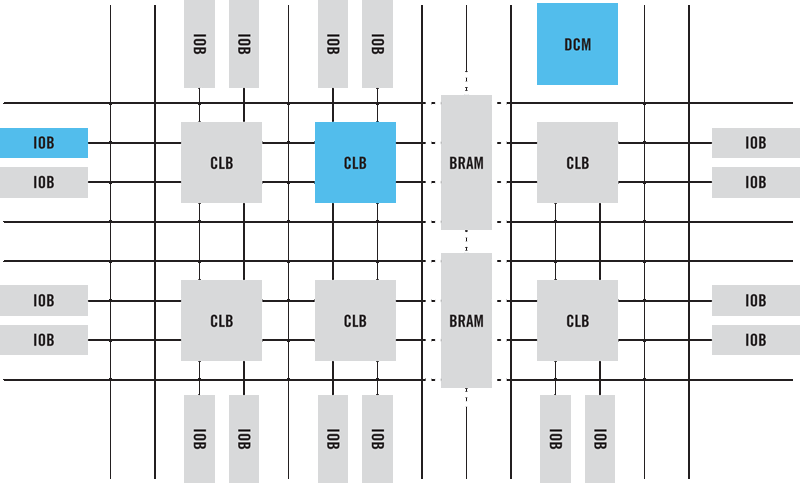
\includegraphics[width=.7\textwidth]{img/fpga-block-structure}
\caption{Structural FPGA overview \cite{xilinxFPGA}}
\label{fig:fpgastructure}
\end{figure}

\begin{figure}
\centering
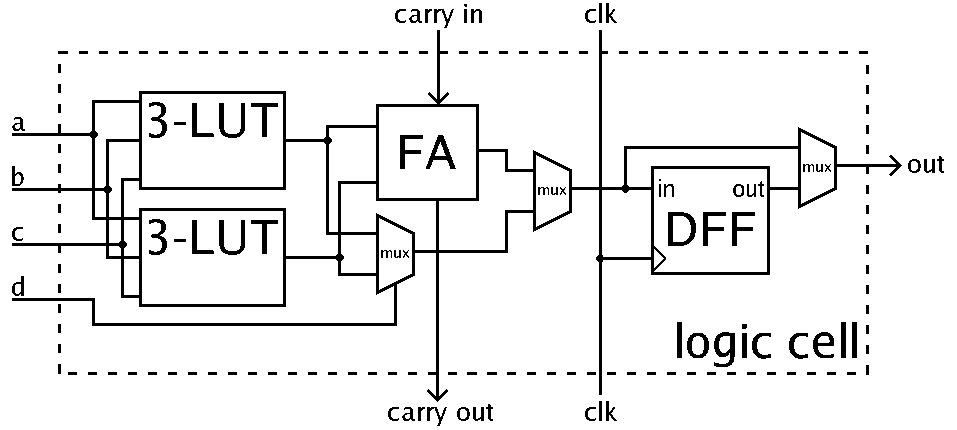
\includegraphics[width=.7\textwidth]{img/fpga-clb}
\caption{FPGA CLB example overview \cite{fpgaclbimg}}
\label{fig:my_label}
\end{figure}



\subsection{I/O capabilities}
A FPGA development board generally includes a number of I/O devices. Simple devices for input include buttons and switches, while simple output devices are generally LEDs or LED displays. Furthermore, a development board often includes a set of pin headers, which can be configured individually to be input or output ports. 

More complex I/O devices are included as well. Such as VGA output controllers, microphone, Ethernet, USB, .... These devices operate within strict timing constraints in order to work properly. This prevents the experiment setup from properly using the device, since it runs on a irregular, low frequency. 

Buffering (right term?) of some types of input, such as push buttons. When a user presses a push button while the experiment is halted, the signal should be artificially set to be high during the next cycle.

I/O devices can only be seen as combinational circuits. I/O devices that are based on sequential logic, such as a LED display controller, an abstraction needs to be created such that the device behaves like a combinational circuit. 

\subsection{Platform dependence}
Earlier approaches that have applied FPGAs in education have resulted in solutions that are very board-specific. FPGAs manufactured by both Xilinx and Altera have been allied in the education of these topics. Both manufacturers have tightly integrated their software development kits with their FPGAs. Development board are manufactured by these manufacturers, as well as third parties, such as Digilent. 

Hardware design projects may be interchangeable between different versions of a FPGA chip, as well as different product families.

\subsection{Programming}
Current FPGAs generally make use of the IEEE 1532 standard for in-system programming, which extends the IEEE 1149.1 'JTAG' boundary scan protocol. In order to program these FPGAs, one makes use of dedicated JTAG programming hardware and software. Such hardware and software is commonly available.  

FPGA development board manufacturers generally integrate JTAG programming hardware in their designs, allowing progamming over a serial connection to their PC, such as USB. Manufacturers combine their development boards with software development kits that facilitate the operating system drivers and software required for the programming process. Other means of programming are seen as well, such as support for USB storage devices or memory cards on which a file is placed that is automatically read by the development board and programmed onto the FPGA. FPGA development boards generally feature a JTAG interface as well, allowing for a custom method of programming using external tools. 

\subsection{PC Communication}
In order to allow for communcation with a PC, FPGA development board manufacturers generally include one or more communication interfaces in their board designs. Many FPGA development boards currently available come with a USB interface over which a virtual serial interface is exposed, commonly known as a virtual COM port. The serial signal is often controlled by a UART implementation that is programmed onto the FPGA. Other examples of communcation interfaces are RS232 and Eternet ports, where dedicated hardware components on the FPGA development board are responsible for translating signal levels controlled in the FPGA to interface standard levels. 

TODO uitleggen waarom synchronous sequential logic niet werkt op FPGAs. Timing sensitive, zeer geavanceerde place \& route. Wordt niet ondersteund door tools. 

% FPGA
% Eductional
% Computer architecture
% PC
% Instruction level view
% MIPS 

% Introduction
% Problem description
% Related work
% Educational softcores
% 
% FPGA fundamentals
% - toolchain
% 

\chapter{Model}

This chapter will propose a model that provides a theoretical solution to the problem statement as described in section \ref{sectionproblemstatement}. This model addresses the problem statement from a technical and architectural point of view, as well as how user processes are affected. As a starting point, a description of a basic model for experiment setups on FPGA development boards is given in section \ref{sectionbasicmodel}, which is then extended and modified through a series of stages. In every stage, a particular aspect of the problem statement is addressed, forming a complete solution eventually. 

In section \ref{sectionvirtualizingio} the possible limiting factor of the  number of I/O devices on the FPGA development board is addressed by introducing the concept of a controller. This controller provides the experiment setup logic with a variable amount of virtual I/O channels. The levels of these I/O channels can then observed and controlled through controller-specific PC software. All of the physical I/O devices are temporarily removed from the model, as well as most of the FPGA's other peripheral devices.

In section \ref{sectioncyclecontrol} the controller is extended such that it allows for cycle-accurate control of sequential experiment setup logic. Users control cycles through the PC software, but the model supports autonomous operation as well. This new functionality is added through expansion of the experiment setup interface.

In section \ref{sectioncontrollerabstraction} the experiment controller's interface is generalized, such that the interface dependencies between experiment setup and controller are removed. This allows for independent development of controllers and experiment setups, allowing for random combinations of board-specific controllers and independent experiment setup logic. The controller's PC interface is generalized as well, which allows for the development of universal PC software.

In section \ref{sectionreintroducingio} the FPGA development board's physical I/O devices are reintroduced into the model, after being removed from the model in section \ref{sectionvirtualizingio}. This step is essential in enabling a student's physical view of the experiment setup and providing a hands-on experience. The development of experiment setups remains an independent process.

% The model addresses the following aspects of hosting hardware experiment setups on FPGA development boards:
% \begin{itemize}
% \item FPGA development board independence
% \item Abstraction of FPGA (development board) manufacturers 
% \item distribution format for experiment setups
% \item Reuse of components 
% \item ease of development
% \item ease of use for students
% \end{itemize}

% Advantages
% \begin{itemize}
% \item Controller abstraction results in experiment setups to be FPGA development board independent
% \item Controller abstraction results in the simplification of design considerations for instructors when developing experiment setups. Instructors only need to consider the experiment setup-controller interface when developing experiments. 
% \item Controller abstraction leads to generalization of testing and verification tools used for experiment setup development
% \item A generic format for experiment setups allows for easy interexchange of experiments
% \item Clear separation of concerns
% \item Abstraction of development boards allows for reuse of board/controller hardware components. 
% \item clear definitions of information exchange formats for experiment setups, board packages, and deployable distributables. 
% \item Generalization of components of the model leads to reuse
% \item Interface of abstract experiment setup is same as generic memory element/block ram, allowing for reuse of exisiting technology. 
% \end{itemize}

% Disadvantages
% \begin{itemize}
% \item Only supports combinational and synchronous sequential logic
% \item Instructors need to implement 'clock\_enable' signal.
% \item Additional complexity is introduced into the toolchain
% \item Abstraction of I/O devices results in loss of functionality and overhead in addressing them as combinational devices. Some functionality of the development board is lost. For example, real-time sensor measurements are impossible on low frequencies. 
% \end{itemize}

% In this section, a basic model is introduced. This model is extended in a series of steps, eventually resulting in this thesis' proposed model.
% \begin{itemize}
% \item Interface
% \item Architecture
% \item Workflow
% \end{itemize}

% Development board requirements
% \begin{itemize}
% \item FPGA that is supported by toolchain
% \item FPGA development board programming interface is supported by student toolchain
% \item Serial communication interface on FPGA development board
% \item (optional) Human interface I/O devices
% \end{itemize}

% The proposed models is supposed to allow for FPGA development boards to provide students a hands-on experience in their hardware logic experiments.

\section{The Basic Model}
\label{sectionbasicmodel}

As a starting point, a description of a basic model for experiment setups on FPGA development boards is given. An overview of the basic model is displayed in figure \ref{fig:overview-basic}. The model features a PC and a FPGA development board as the two primary physical components. An interface between the PC and the FPGA development board exists over which the board exposes the \texttt{Board.Program()} operation. This operation initializes the FPGA by loading the contents of a FPGA-specific bitstream file and configuring the FPGA's components. The physical and electrical characteristics of this interface are considered to be irrelevant and may even be a process that involves manual user operations, such as transferring a memory card.

\begin{figure}[h]
\centering
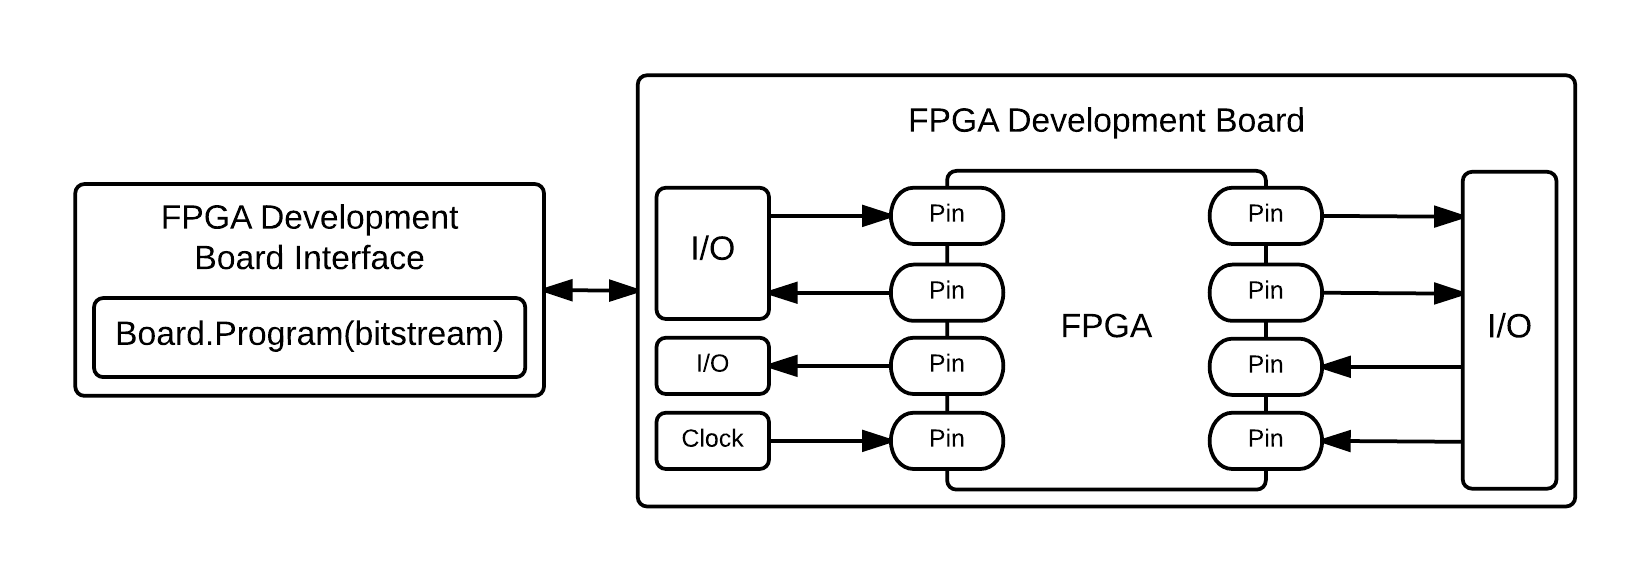
\includegraphics[width=0.8\textwidth]{img/overview-basic}
\caption{The basic model, an overview of the FPGA development board and its exposed interfaces.}
\label{fig:overview-basic}
\end{figure}

In this basic model, the FPGA development board is considered to be a printed circuit board (PCB) which hosts and interconnects a FPGA and its various peripheral components. Not all pins of the FPGA package and not all peripheral devices are considered to be relevant to the model. Only the pins whose signals can be controlled through the FPGA's contained logic are included. Peripheral devices that do not connect to these pins, such as power supplies or programming circuits are excluded from the model. Specifically, the presence of a clock generating device is assumed, providing the FPGA with a clock signal on one of its pins. Although this model is a great simplification of reality, this abstract view is assumed to be sufficient for the purposes of this model and applicable to most FPGA development boards. 

Besides the omission of details of the FPGA's peripherals, a part of the FPGA's internal complexities are hidden from the model as well. Figure \ref{fig:fpga-basic} gives a graphical overview of the FPGA's internals and its contained logic. The FPGA's internal interface is simplified and defined to be a container for the end product of a HDL developer's work: an entity with input signals, output signals and an input clock signal. Other physical, electrical or logical characteristics of the FPGA are not included in the model.

\begin{figure}[h]
\centering
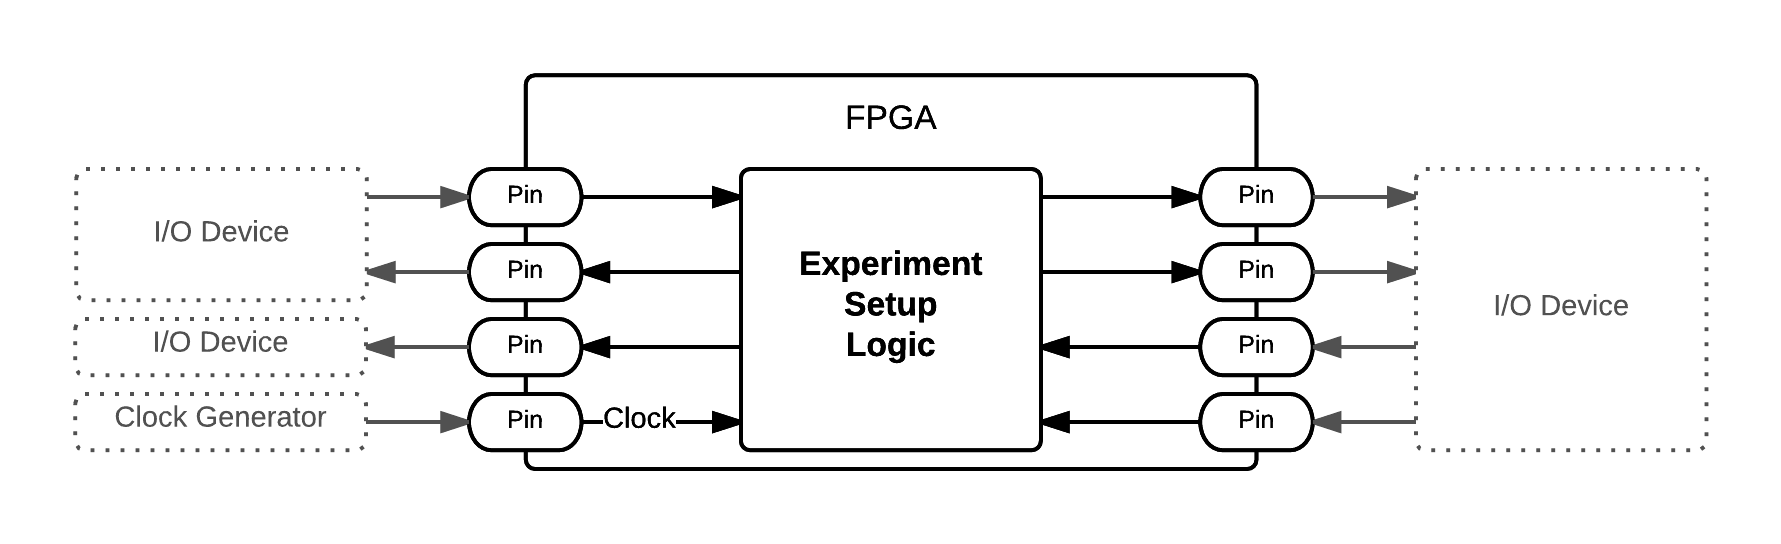
\includegraphics[width=\textwidth]{img/fpga-basic}
\caption{The basic model, an overview of the FPGA and its contained experiment setup logic. No specific architecture is applied to the logic.}
\label{fig:fpga-basic}
\end{figure}

In the case of this basic model, no specific architecture is defined that will embed the experiment setup logic into the FPGA development board. A specific architecture will be developed in the following stages. At this stage of the model, a developer is responsible for the development of its own architecture that embeds the experiment setup logic into the environment of the FPGA.

In this basic model, two user roles are defined: experiment setup developers and experimenters. In a classroom environment, an instructor can be considered an experiment setup developer and a student can be considered an experimenter. 

\subsection{Experiment Setup Developers}
\label{sectionexperimentdevelopers}
Experiment setup developers are responsible for the design, implementation, testing, documentation and distribution of experiment setups for use on FPGA development boards. The end product of their work is a software package that contains a bitstream file and optionally the source files used in the bitstream file's compilation process. Figure \ref{fig:process-development-basic} displays a graphical overview of the experiment setup development process. 

\begin{figure}[h]
    \centering
    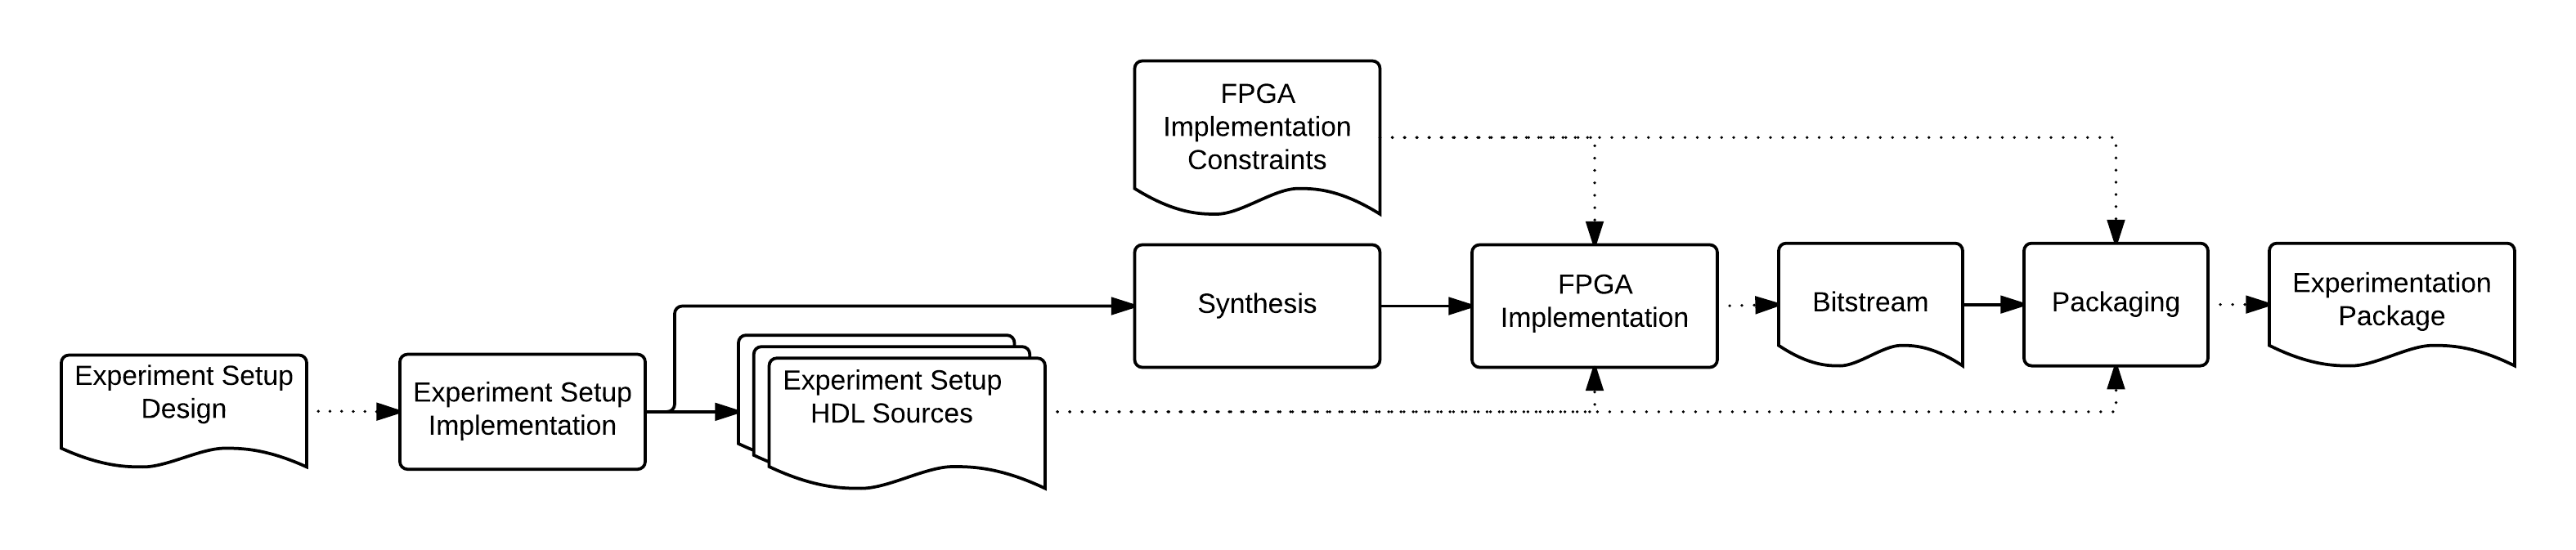
\includegraphics[width=\textwidth]{img/processes-basic-development}
    \caption{The basic model, an overview of the experiment setup development process.}
    \label{fig:process-development-basic}
\end{figure}

As shown below, an experiment setup developer must have knowledge of a significant number of subjects and technologies: 

\begin{itemize}
\item Designing an experiment setup requires knowledge on the subject of digital logic and digital systems. 
\item For the design to contain meaningful educational content, the developer should have experience in teaching the subject. 
\item Translating the design into a working, valid implementation in VHDL or Verilog requires experience in HDL development.
\item Embedding the implemented design in a FPGA development board requires knowledge of the specific FPGA, its development tools and the FPGA's peripheral devices.
\end{itemize}

\subsection{Experimenters}

Experimenters are responsible for carrying out experiments. They obtain experiment setup software packages and initialize experiment setups on their FPGA development boards. In order to complete the experiment, they make observations and interact with the experiment setup that is contained within the FPGA. Figure \ref{fig:process-experimentation-basic} displays a graphical overview of the experimentation process. In this basic model, two different methods of interaction are defined: interaction through board I/O devices and interaction through the process of HDL source modification, recompilation and reprogramming. Observation of the experiment's results can be done through the FPGA development board's I/O devices. Some development tools allow for live inspection of the FPGA's internal signal levels through a PC connection.

\begin{figure}[h]
    \centering
    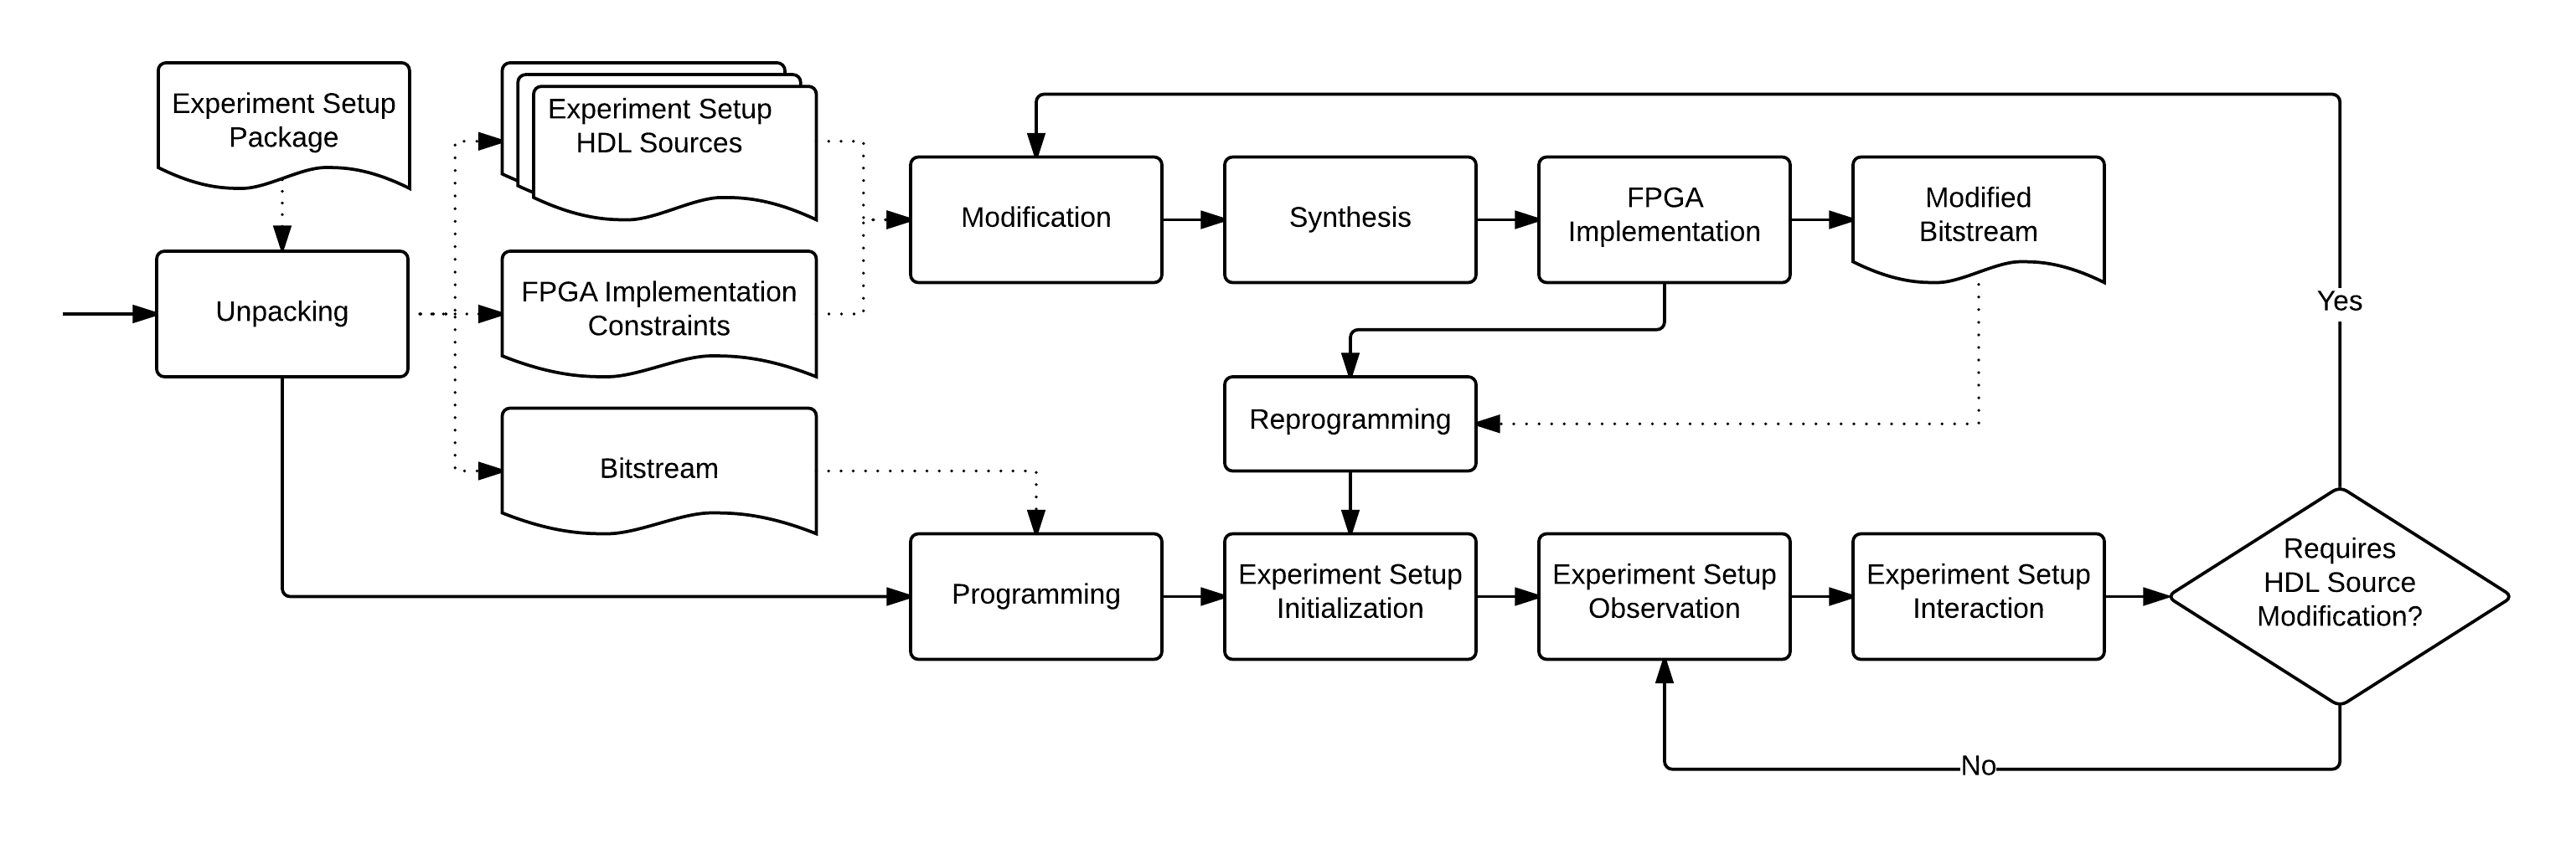
\includegraphics[width=\textwidth]{img/processes-basic-experimentation}
    \caption{The basic model, an overview of the experimentation process.}
    \label{fig:process-experimentation-basic}
\end{figure}

In order for a user to act as an experimenter, one must understand the logic and workings of the obtained experiment setup. Furthermore, an experimenter must understand the basic concepts and role of the FPGA development board, as well as how to program the FPGA via the experimenter's PC. In preparation of the experiment, experimenters must install programming software and operating system drivers for the FPGA development board. In this case, interaction and observation is done through the board's I/O devices. 

Including the PC as a tool for observation and interaction requires additional knowledge and preparation from experimenters. In order to understand and modify the experiment setup's HDL sources, users must be familiar with the programming language used. Recompilation requires users to install and understand the FPGA's development tools in order to set up a proper development environment. Furthermore, this method of interaction will significantly increase the time required for every change to be processed, since the process of recompilation is a slow process. Using the FPGA as a tool for observation requires further familiarization with the FPGA's development tools.







\section{Virtualizing I/O}
\label{sectionvirtualizingio}
Regular FPGA development boards offer a limited set of I/O devices. As a consequence, this allows for observation and control of experiment setup logic entities with a limited number of input and output signals. Embedding entities with a large number of inputs and outputs however, requires a different approach. 

In order to support experiment setup entities with a large number of input and output signals, the basic model's logic architecture is extended through introduction of the controller. Figure \ref{fig:fpga-inout} gives an overview of the FPGA and the newly defined architecture. The experiment setup entity's inputs and output signals are available to the controller only, but both components still share a common clock signal. The signal levels of the FPGA's peripheral devices are no longer driven by the experiment setup entity. Following the previous section's criteria, these devices are considered irrelevant and thus removed from the model. Only the clock generating device and a single machine-machine communication device remain part of the model. 


\begin{figure}[h]
\centering
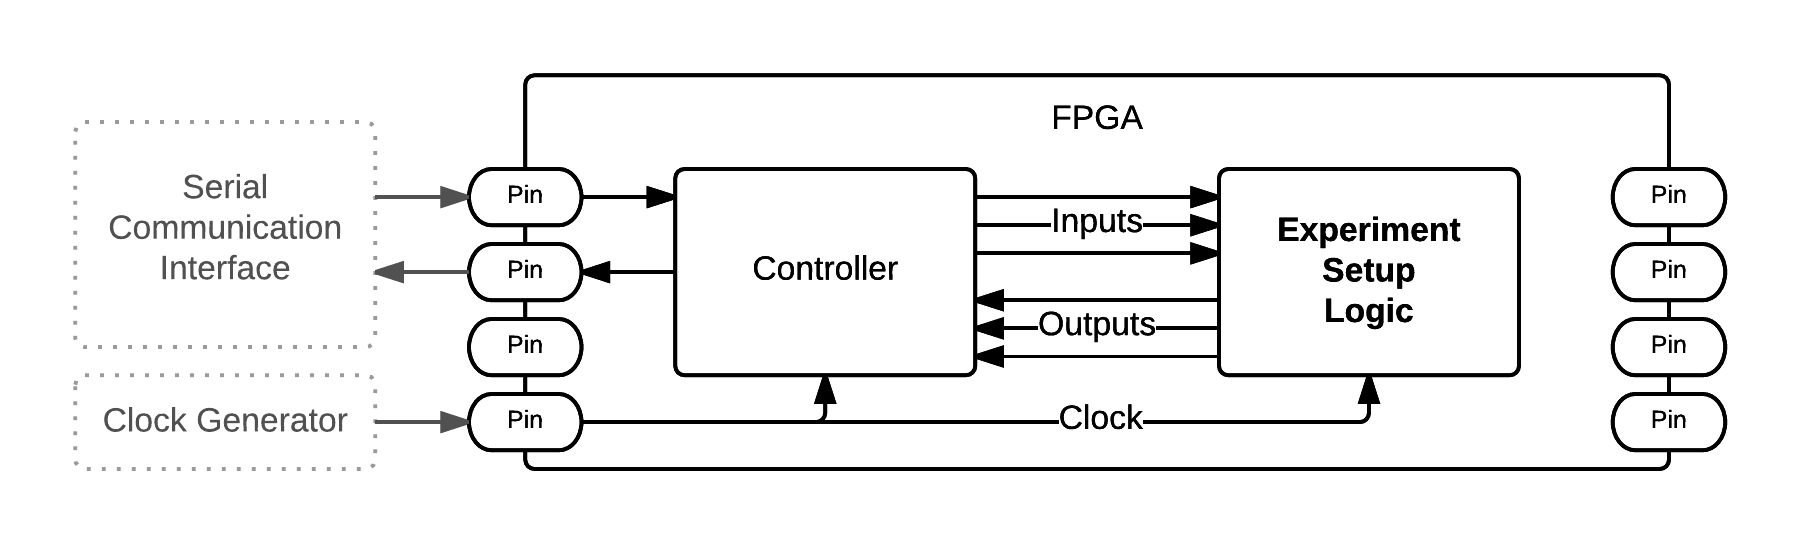
\includegraphics[width=\textwidth]{img/fpga-inout}
\caption{I/O virtualized, an overview of the FPGA and its contained logic architecture. The controller embeds the experiment setup logic into the FPGA.}
\label{fig:fpga-inout}
\end{figure}

The controller is a component that acts as an intermediary between the experiment setup logic and an experimenter's PC. The experiment setup's state is observed and controlled through controller-specific software, a method also presented in \cite{holland2003harnessing} and \cite{bulic2013fpga}. A hardware-based method to observe and control the experiment setup's state is described in \cite{al2007teaching}. A software-based solution however, does not increase the cost of the experiment. Furthermore, a software-based approach will allow for more flexibility, as shown in the following sections. 

The controller exposes an additional interface through a communication channel that must be provided by one of the FPGA development board's communication devices, as can be seen in figure \ref{fig:overview-inout}. This interface defines operations that allow for the experiment setup entity's individual input and output signals to be controlled and observed respectively. A similar interface for observation and control of specific signals is described in \cite{holland2003harnessing}. 

\begin{figure}[h]
\centering
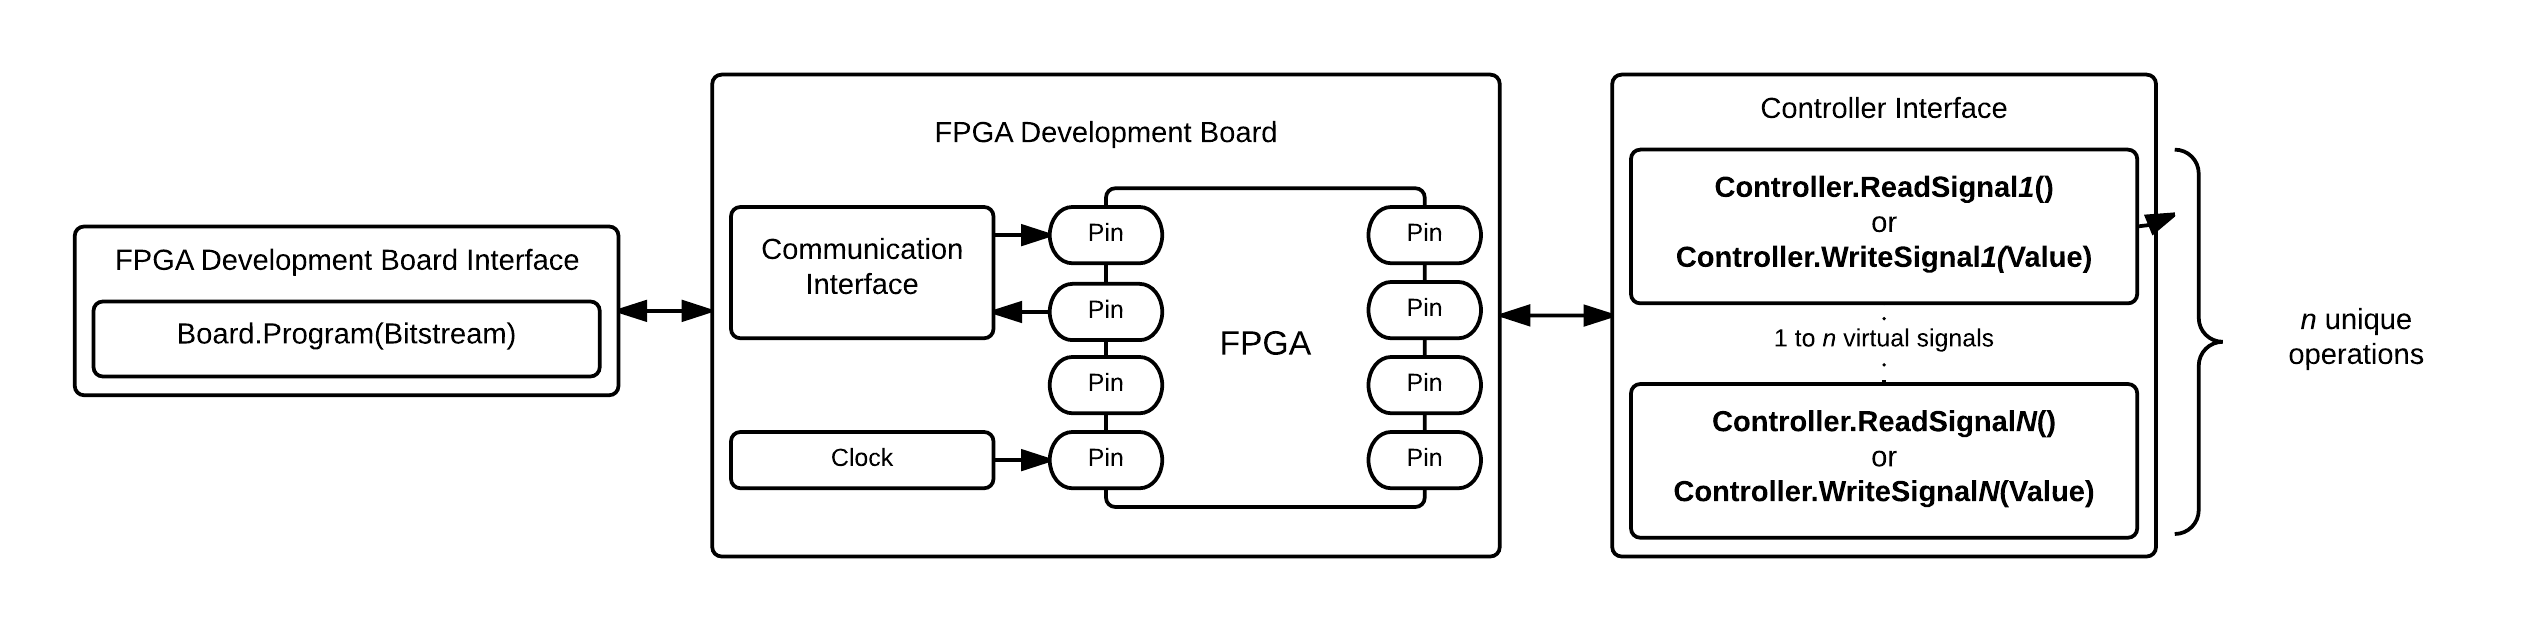
\includegraphics[width=\textwidth]{img/overview-inout}
\caption{I/O virtualized, an overview of the FPGA development board and its exposed interfaces.}
\label{fig:overview-inout}
\end{figure}

The explicit separation of concerns in the logic architecture allows for separate implementation and validation processes for experiment setup logic, controller logic and PC software. This partitioning subsequently allows for distribution of work among specialists, removing the need for a single experiment developer to have knowledge and experience in all the areas previously described in section  \ref{sectionexperimentdevelopers}. As a consequence of the separation however, more dependencies are introduced into the development process. The development of a controller component requires a definition of the experiment setup's interface and any change in this interface definition requires modification of the controller. A similar dependency exists between the controller and the PC software. A change in the experiment setup entity's interface definition will thus not only result in the need for modification of the controller, but in the need for modification of the PC software as well. These dependencies are addressed and removed from the model in section \ref{sectioncontrollerabstraction}.

Experiment setup interaction through dedicated PC software will simplify the experimentation process for experiment setups with large number of input and output signals. Involving the PC removes the need for experimenters to install and familiarize themselves with the FPGA's development tools. Experimenters will be able to interact with the experiment setup through a graphical interface on the PC, removing the need need for HDL programming skills and allowing for real-time interaction, since no recompilation is required. Since the board's I/O devices have been removed at this stage of the model, there is no possibility for users to physically interact with the experiment. The PC software provides the only means of interaction with the experiment setup. These removed I/O devices however, will be reintroduced into the model in section \ref{sectionreintroducingio}.

% TODO Hoe ziet de PC software er uit?



\section{Cycle control}
\label{sectioncyclecontrol}
In the previous section, the basic model has been extended to include a definition of the controller. This controller allows for the embedding of experiment setup entities with an arbitrary number of input and output signals that are defined through combinational logic. FPGAs in general lack practically useful support for containment of asynchronous sequential logic, but the availability of a clock signal in the current model does provide support for experiment setup entities that are defined through synchronous sequential logic. However, this clock signal is constant and cannot be varied in speed or temporary stopped. Embedding an experiment setup entity of synchronous sequential logic at this stage of the model would result in an uncontrollable situation of continuous state changes at high speed. This limited control over the clock signal is due to the nature of how FPGAs work and prevents cycle-accurate interaction with the experiment setup. In order to be capable of cycle-accurate observations and control over synchronous sequential experiment setup logic, the model requires further extension.

\begin{figure}[h]
\centering
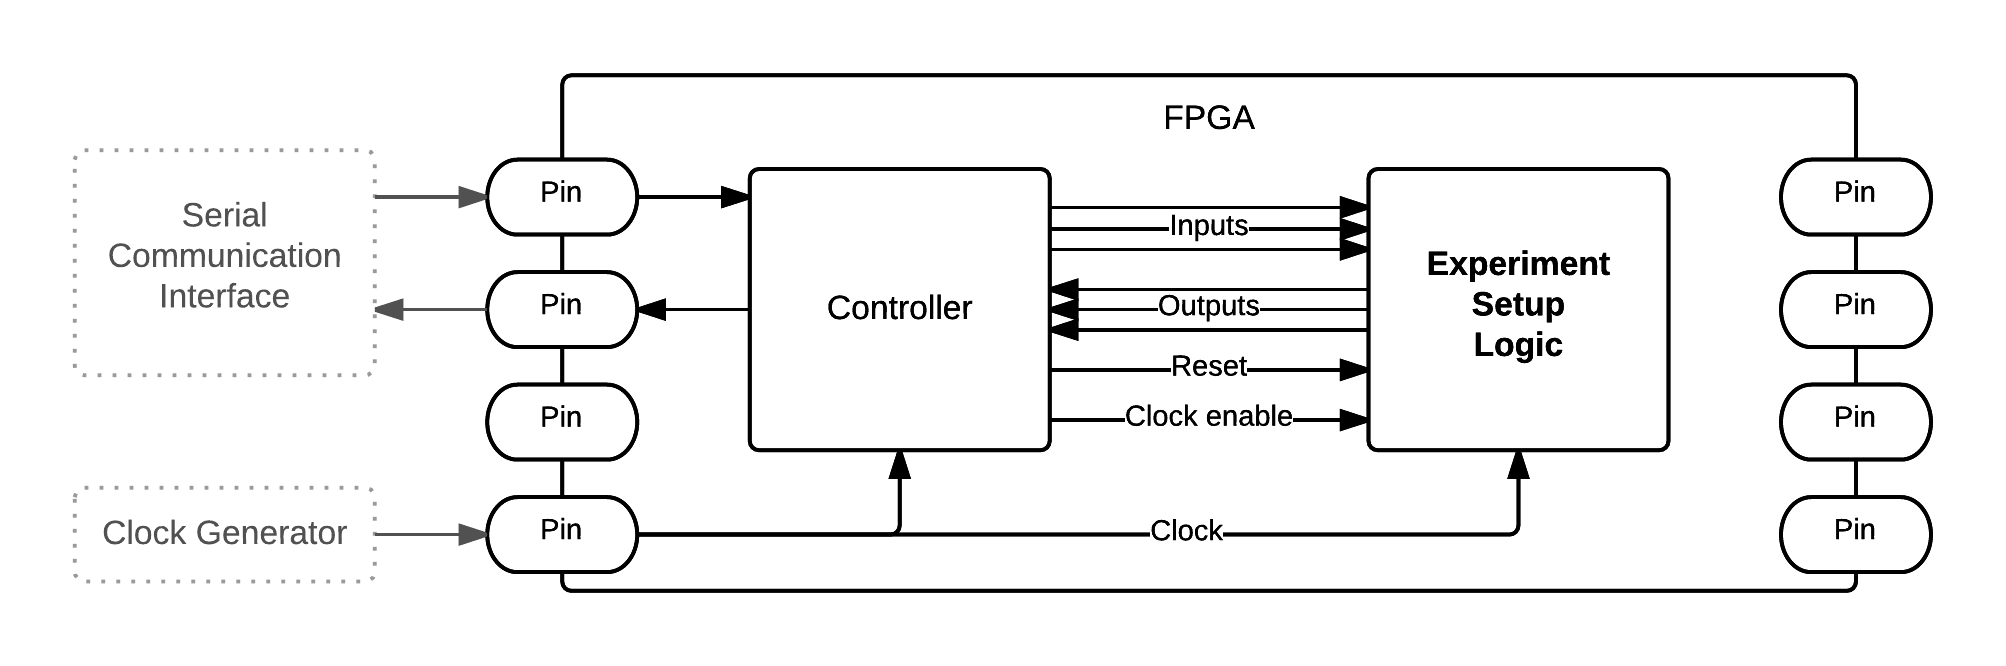
\includegraphics[width=\textwidth]{img/fpga-control}
\caption{Cycle control, an overview of the FPGA and its contained logic architecture. The \texttt{clock\_enable} and \texttt{reset} signals are added to allow for cycle-accurate interaction and (re)initialization.}
\label{fig:fpga-control}
\end{figure}

As a solution to the problem stated above, the FPGA's contained logic architecture has been extended, as displayed in figure \ref{fig:fpga-control}. The most significant change is the addition of the \texttt{clock\_enable} input signal on the experiment setup's interface definition. Combined with the \texttt{reset} signal, these new input signals allow for cycle-accurate control and reinitialization of the experiment setup logic's state. The introduction of the \texttt{clock\_enable} signal will require modification of every synchronous memory element present in the experiment setup logic, as displayed in figure \ref{fig:clock-manipulation-enable}. By multiplexing the input signal for every memory element based on the same \texttt{clock\_enable}, one can control the state change in a cycle-accurate manner. The method of using enable signals to control synchronous logic is described in \cite[Sec 2.4.5]{arora2011art}.

One may argue that this approach is unfavourable, since it requires modification of existing experiment setup logic designs. This method for controlling state change however, is a common approach in FPGA-targeted HDL development and is used in many designs. More specifically, this approach was also taken in controlling the experiment setups described in \cite{holland2003harnessing} and \cite{bulic2013fpga}. As stated before, FPGAs do not allow for dynamic manipulation of clock signals by design, a method known as clock gating (figure \ref{fig:clock-manipulation-gated} ). Clock signals are distributed over the FPGA through dedicated lines that cannot be altered through HDL logic. Some manufacturers include support for static clock division, but still only down to relatively high speeds and do not allow for dynamic adjustment of clock speed [TODO: Bron]. 

% Opmerking Taco 
% Opmerking bij fig 3.8 discussie. Het board dat je gebruikt is een artix7
% en die familie (d.w.z. de "7" familie van xilinx) gedraagt zich anders. Er kunnen verschillende clockdomeinen gebruikt worden en dan
% heb je wel degelijk een soort van gated clock, hoewel dat nooit gebeurt via clk_gated = clk_org &
% enable. Lees het 7 series fpga clocking resources user guide document van xilinx!

\begin{figure}[h]
    \centering
    \begin{subfigure}[t]{0.5\textwidth}
        \centering
        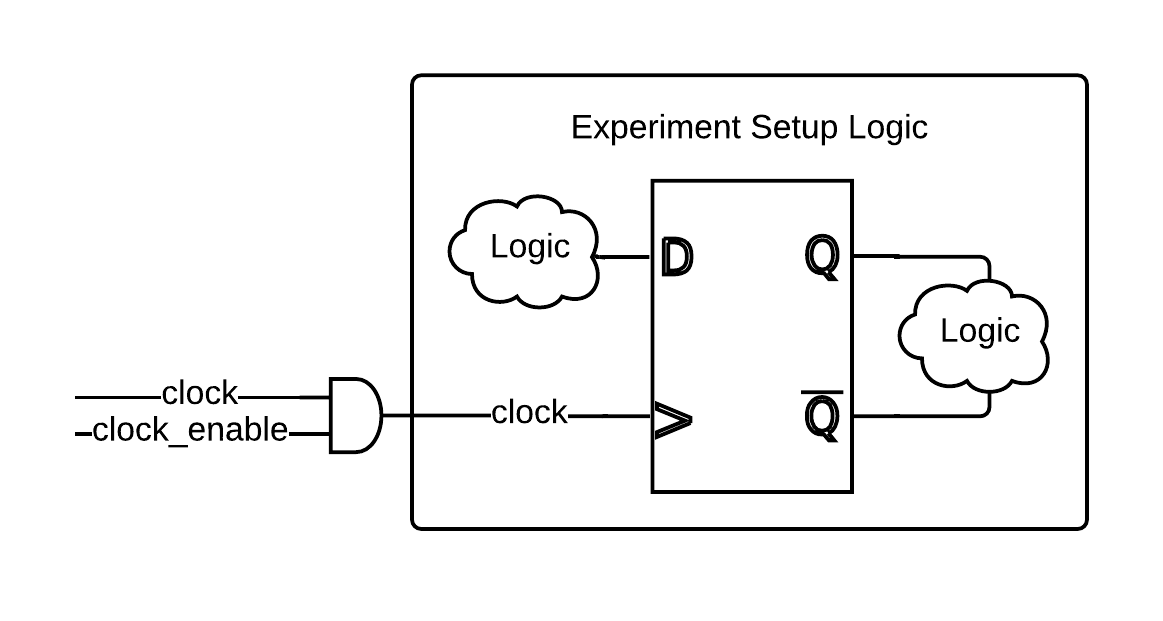
\includegraphics[height=1.5in]{img/clock-manipulation-gated}
        \caption{Gated clocks}
        \label{fig:clock-manipulation-gated}
    \end{subfigure}%
    \begin{subfigure}[t]{0.5\textwidth}
        \centering
        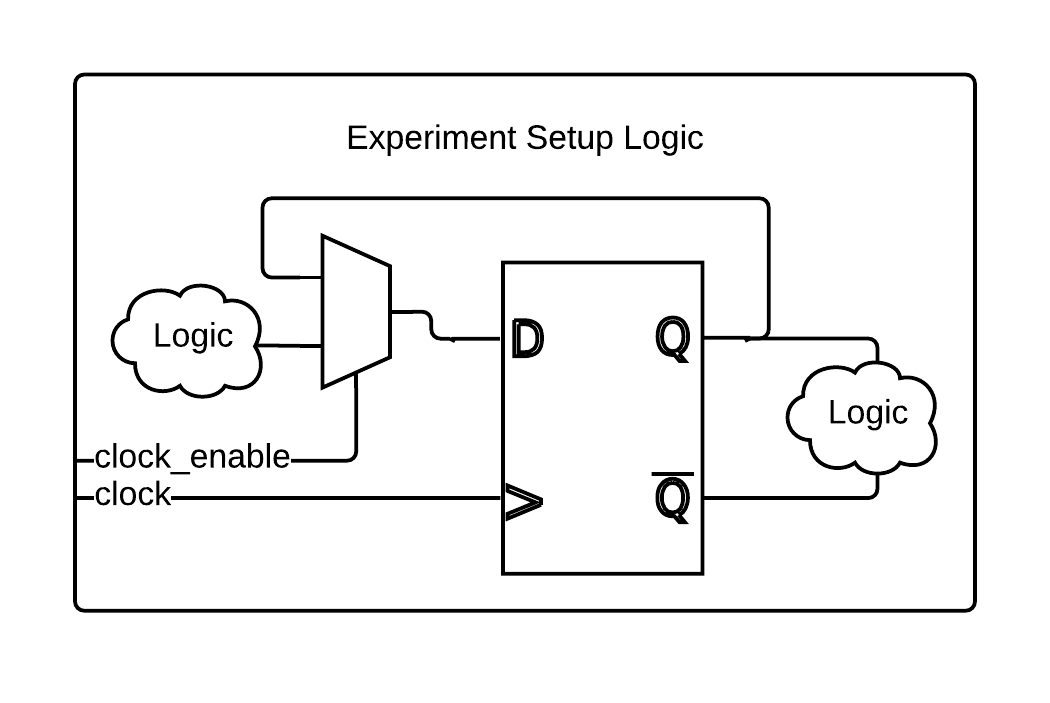
\includegraphics[height=1.5in]{img/clock-manipulation-enable}
        \caption{Enable signal}
        \label{fig:clock-manipulation-enable}
    \end{subfigure}%
    \caption{Controlling state transitions through a clock enable signal and a gated clock signal. FPGA's do not support gated clock signals.}
    \label{fig:clock-manipulation}
\end{figure}

In order to make this newly developed functionality available to the experimenter through the PC software, the controller interface is extended to support new operations that allow for the control of cycles. As displayed in figure \ref{fig:overview-control}, five new operations are available through the controller's interface. The \texttt{Controller.Reset()} operation (re)initializes the experiment setup to it initial state and waits for the next operation. Experimenters have manual control over the experiment setup's cycles through the \texttt{Controller.Step()} operation. The controller may also be instructed to manage the experiment setup autonomously through the \texttt{Controller.Start()} operation. The maximum operating frequency may be defined through the \texttt{Controller.LimitSpeed()} operation. The \texttt{Controller.Stop()} operation stops the controller's autonomous management of the experiment setup and awaits the next operation. Similar interfaces for cycle-accurate control of experiment setups are described in \cite{holland2003harnessing} and \cite{bulic2013fpga}.

\begin{figure}[h!]
\centering
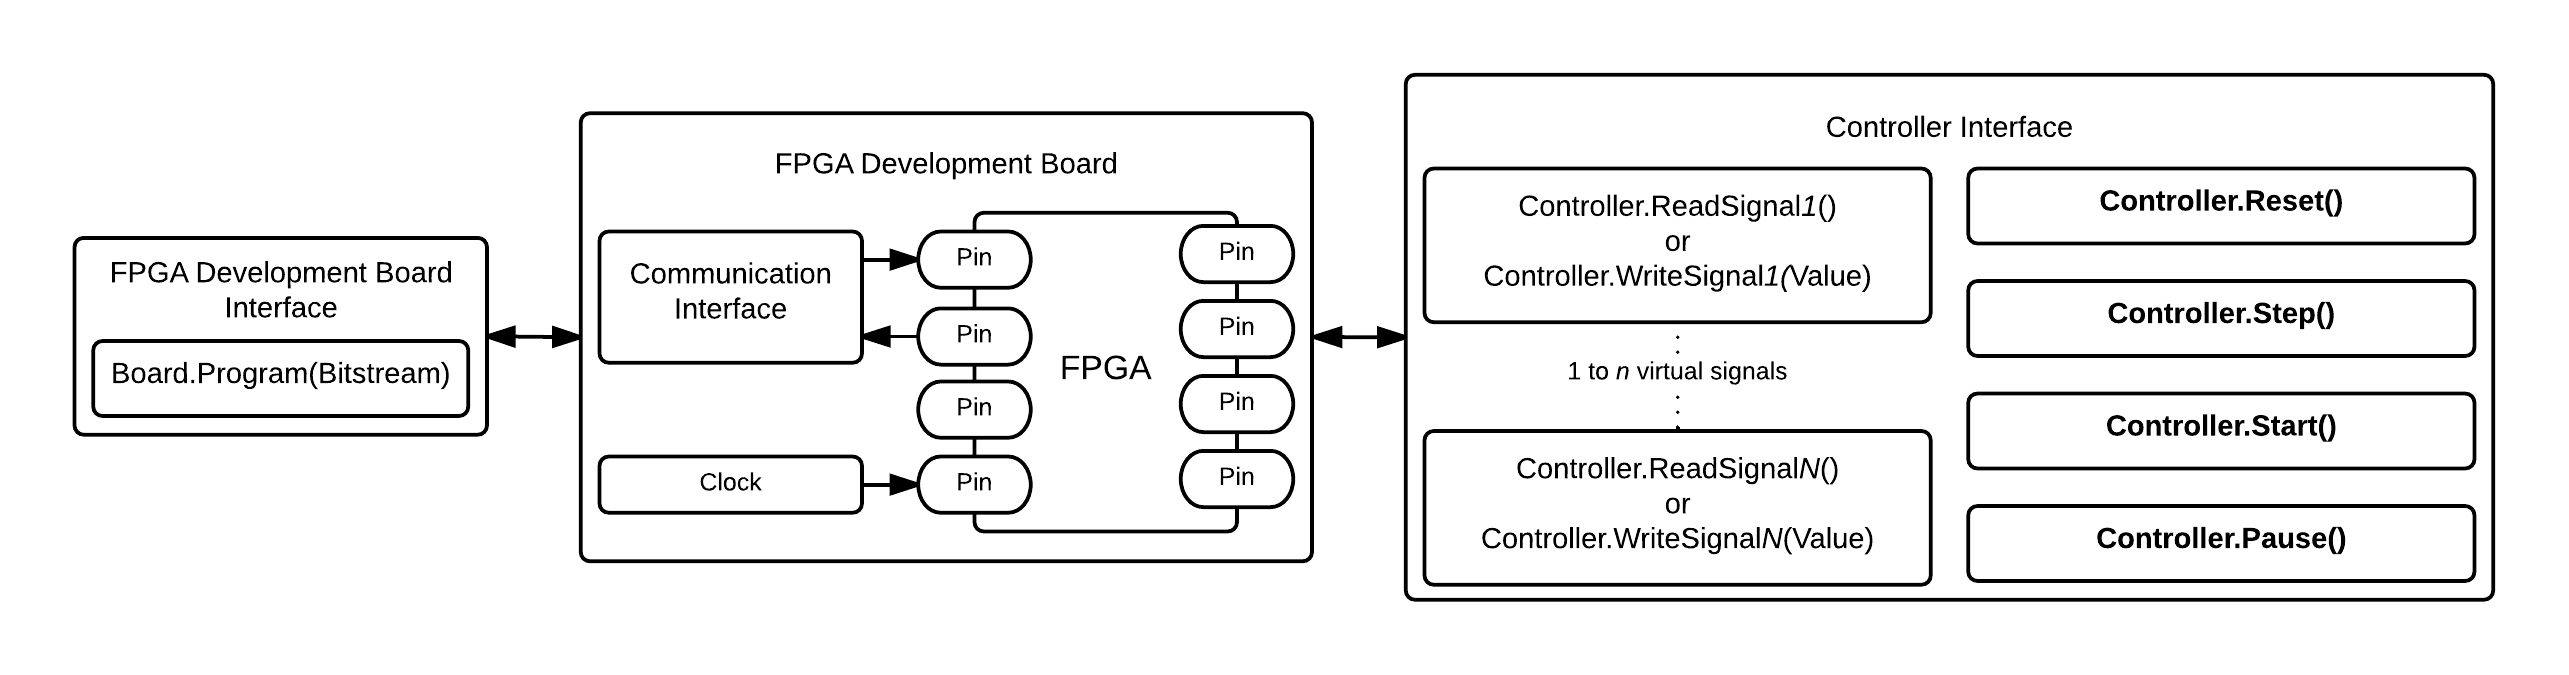
\includegraphics[width=\textwidth]{img/overview-control}
\caption{Cycle control, an overview of the FPGA development board. The controller's interface is extended with operations that allow for cycle-accurate interaction with the experiment setup.}
\label{fig:overview-control}
\end{figure}



% TODO: Students must be able to disconnect from the PC and consider the setup as an autonomous entity. The controller interface needs to be extended with a PLAY/PAUSE instruction as well as a means to set the experiment setups clock speed. There needs to be the distinction between a slave mode when connected to the pc as well as a autonomous mode when disconnected.


% \subsection{FPGA Clock management}
% FPGAs generally run on a single clock signal. On modern FPGAs, this clock signal has a frequency in the order of megahertz, which would result in the execution of the experiment at millions discrete steps per second. This clock is generally fixed. In order for students to be able to control their clock speed or even pause their experiment for observations, a second signal must be introduced into the experiment, allowing the enabling of a clock signal. By enabling this 'clock enable' signal for the duration of one clock cycle, the experiment progresses one discrete time step. A disadvantage of this approach is that experiments must be adapted to support this method of managing clocks. This approach however is commonly seen in industry IP components.

% DCM is unsuitable, because it does not allow for halting of the clock signal as well as running on very low frequencies.

% Experiments requiring async clocks can fake this behaviour by deriving a 'clock enable' using a counter.

% See figure \ref{fig:fpga-control}.







\section{Board Component Abstraction}
\label{sectioncontrollerabstraction}

The controller does no longer provide an interface to the experiment setup, but acts as a proxy to control the experiment setup's interface. This does not only allow for a reuse of controlling logic, but a simplification as well, since the interface that is exposed to the controller is simplified as well.

At this stage of the model's development, it supports the embedding of experiment setups defined through combinational logic as well as synchronous sequential logic. Experimenters can interact with these experiment setups through PC software that is specifically developed for the experiment setup. While the model has developed to address a number of problems encountered by experimenters, the problems experienced during development have only been addressed partially. Although an architecture for the FPGA's contained logic was developed in the previous sections, a series of dependencies can still be identified in the development process, as displayed in figure \ref{fig:dependencies-control}.  

The source of these dependencies is the interface between controller and experiment setup. This interface is specific for every experiment setup. By defining a standard interface between experiment setup and controller, this dependency is removed. In the current approach, the experiment setup is considered an entity with inputs and outputs, supplemented by a clock signal, a clock\_enable signal and a reset signal. 

\subsection{Address Space}
%TODO zinnen verbeteren, nog redelijk vaag
% TODO waarom is de keuze voor het model van een address space een goede keuze?
In order to be able to provide a generic interface between controller and experiment setup logic, the experiment setup's interface is modified such that it resembles the interface of a block ram, as can be seen in figure \ref{fig:interface-experiment}. The experiment setup's signals are projected on the address space. 

Losing the information about which signal is which is irrelevant to proper operation of the controller. In order for the PC software to be of any practical use however, a definition of this memory space is required, such that the individual signals can be identified from the memory space. 

\subsection{Interface}
% TODO waarom is een BRAM interface een goede keuze?
%  - eenvoud
% TODO wat zijn de verschillen/voordelen/nadelen t.o.v. andere businterfaces zoals wishbone, AXI etc.
% - wishbone zou een goede optie kunnen zijn ivm open source
% - hoge leercurve bus interfaces
% - master slave interface is voldoende
% - bus interfaces zijn vaak nodeloos complex
% - begrip interface is wijdversprijd
% - ik had niet de capaciteiten om uitgebreid de mogelijke aanvullende voordelen van een businterface te bestuderen, terwijl deze interface voldoende biedt.

\begin{figure}[h]
    \centering
    \begin{subfigure}[t]{0.5\textwidth}
        \centering
        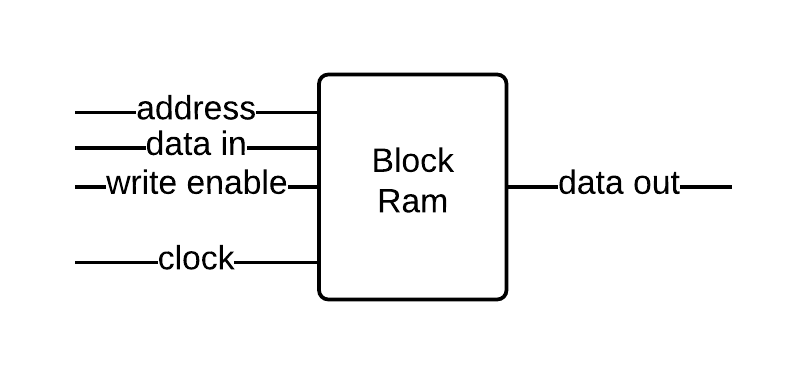
\includegraphics[height=1.2in]{img/interface-bram}
        \caption{Single-port block ram, derived from \cite{RAMs68}}
        \label{fig:interface-bram}
    \end{subfigure}%
    \begin{subfigure}[t]{0.5\textwidth}
        \centering
        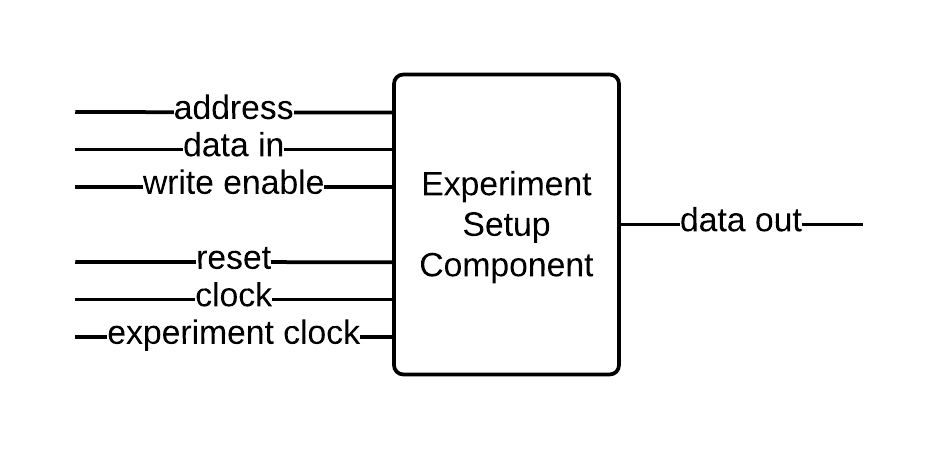
\includegraphics[height=1.5in]{img/interface-experiment}
        \caption{Experiment setup interface}
        \label{fig:interface-experiment}
    \end{subfigure}
    \caption{Interfaces}
    \label{fig:interfaces}
\end{figure}


\subsection{Memory devices}
%TODO sectie verbeteren, nog erg vage zinnen.

The experiment setup has been considered to be an entity with input output signals. Any memory elements contained within the experiment setup can be made accessible through these input and output signals. This solution is not very scalable however. In order to allow for the controller to read and write to large memory elements such as block rams and register files, a different solution is required. A solution to this problem is displayed in figure \ref{fig:logic-wrap-extended}. 

A simple wrapper can be computer-generated in many cases. If complex memory devices are contained within the experiment setup, a wrapper can be defined manually, using an experiment setup adapter component, address space splitters and memory interface multiplexers. 

Large memory elements such as register files and block rams may be defined in HDL. During the compilation process, these elements are infered from HDL code and the FPGA's internal block rams are used. 

% If more memory space is required however, external memory devices such as DDR RAM IC's may be required. Since these external RAM devices require a number of cycles in order to accress the data, they must be abstracted in order to be accessible from within the experiment setup logic. In order to achieve the desired effect of seeing these DDR RAM devices as block ram devices that only require a single clock cycle to operate, the controller must stall the \texttt{clock\_enable} signal until the DDR controller finishes the desired operation. 


\subsection{Composition Process}
In stead of the distinction between controller and experiment setup, a new separation is defined in the controller's logic architecture. A distinction is made between the logic that is targeted to a specific FPGA development board and the logic that targets the standard board component interface. Figure \ref{fig:fpga-abstract} displays this distinction. This distinction is made, because the experiment setup is no longer being defined by it's primary logic, but as secondary interfacing logic as well. 

% The controller was defined to be a specific implementation embedding a specific experiment setup into a FPGA development board.

\begin{figure}[h]
\centering
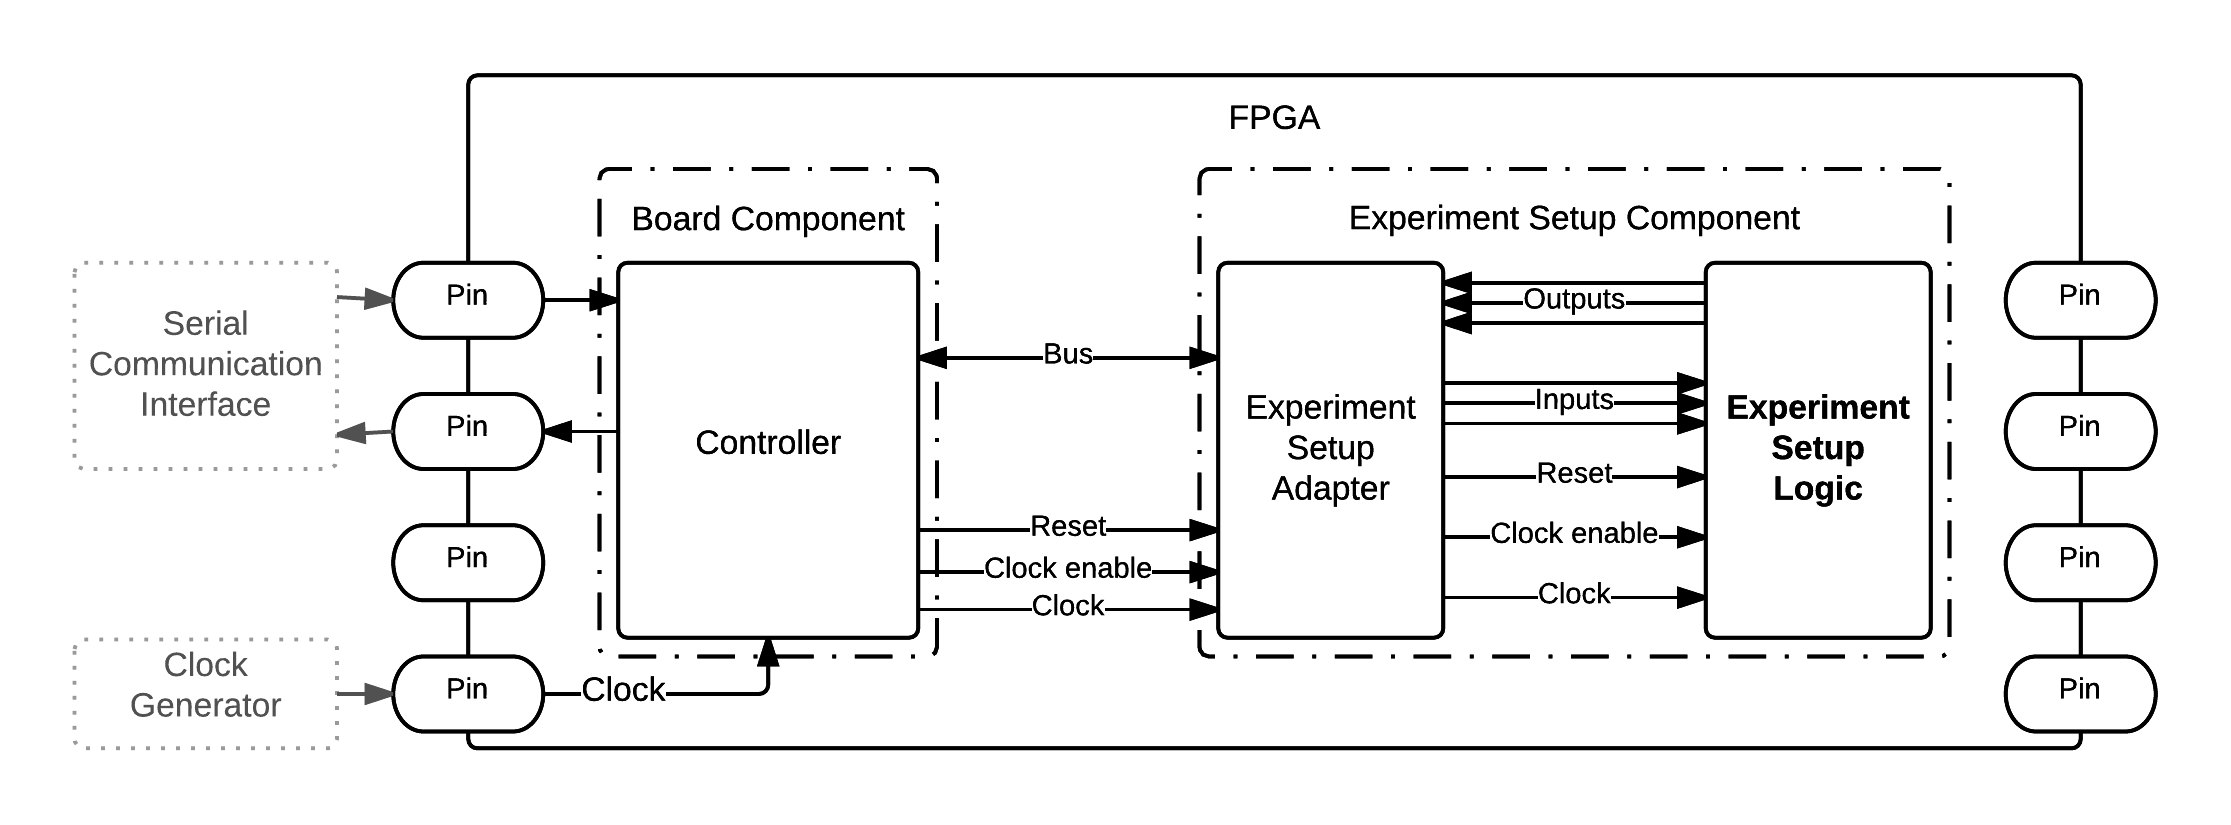
\includegraphics[width=.8\textwidth]{img/fpga-abstract}
\caption{Controller abstracted, FPGA logic design}
\label{fig:fpga-abstract}
\end{figure}

A new process is defined for the composition of board component and experiment setup component into a bitstream file. This results in the processes of experiment setup development and board component development to become independent. Figure \ref{fig:dependencies-abstract} displays the composition process and its relation to the  development processes for experiment setup component and board development component in terms of dependencies. 

\subsection{Experiment Setup Adapter}

In order for an experiment setup logic to conform to the experiment setup component's interface, a component is introduced that acts as an adapter. This experiment setup adapter is a logic component that projects the experiment setup's input and output signals onto an address space. Figure \ref{fig:fpga-abstract} displays the experiment setup adapter.




\subsection{Generic PC Software}
A major advantage of the generic interface between the controller and experiment setup is that PC software can be developed that is no longer specifically tied to one particular experiment setup design. The controller now acts as a proxy between the PC and the experiment setup. The experiment setup is considered an address space from the PC software, no longer an entity with inputs and outputs. In order for this address space to be of any significant meaning, the PC software requires information on how the data in this address space is structured. During the wrapping process a file will be generated, describing how the experiment setup's signals are projected onto its address space. 

% iets zeggen over de faciliterende interface tussen PC en 



\begin{figure}[h]
\centering
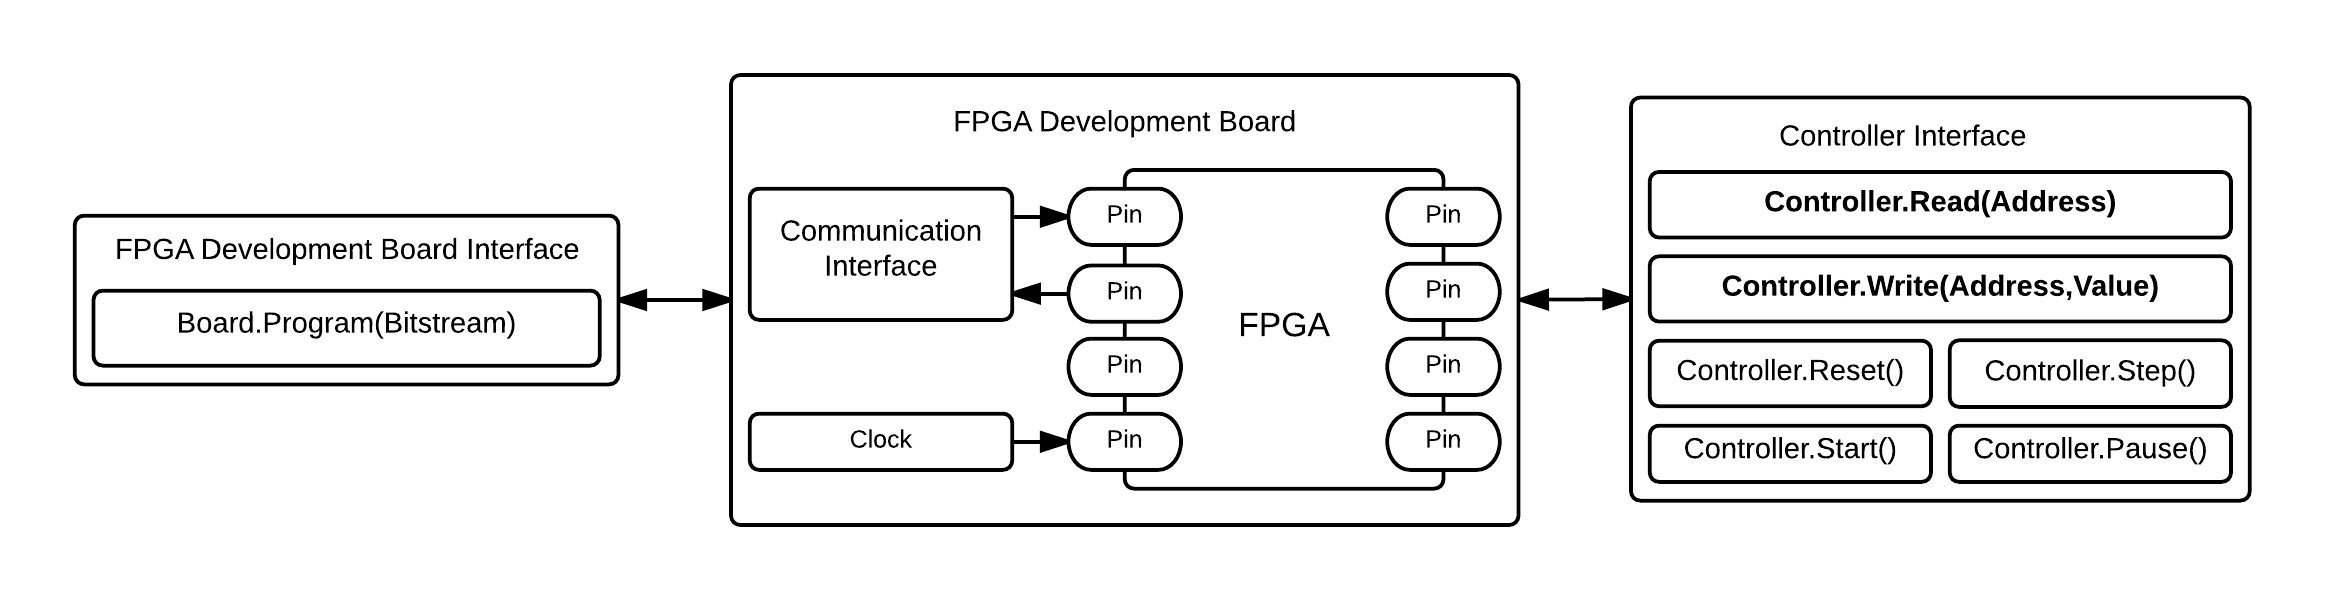
\includegraphics[width=\textwidth]{img/overview-abstract}
\caption{Controller abstracted, overview}
\label{fig:overview-abstract}
\end{figure}


%variable address width
%variable data width

% studenten:
% - nog niet mogelijk snel te switchen
% docenten
% - afhankelijkheden tijdens ontwikkelproces.
% - 

% het is nog niet mogelijk te interfacen met complexe state devices in 


% Developed experiment setups are still board-specific

% Software is still controller-specific

% Controller-specific software

% Experiment-specific controller

% abstraction Allows for reuse of code

% abstraction allows for board-independent experiment development

% abstraction allows for random combination of experiment and controller, allowing for reuse of experiment code

% introduction of standard interfaces removes dependencies from development process

% Removing the dependency from controller to experiment, generic interface.

% Allows for reuse of generic board components for different experiment setup components.

% Complicates experiment development, but process of wrapping can be automated

% view of experiment as address space allows for easy interface from software address space allows for projection of signals as well as memory elements.









\section{Reintroducing Board I/O}
\label{sectionreintroducingio}

Experiment setup has no accurate notion of time, so I/O devices can only be addressed as combinational devices. I/O device drivers facilitate this.

Board I/O capabilities are of vital iportance in providing a physical hands-on experience. Although the FPGA itself is a physical object, the board's I/O capabilities expose the hardware setup's physical behaviour and provide real life interaction capabilities. Without this step, the whole point of a physical hands-on experience is lost.

See figure \ref{fig:fpga-io}

\subsection{I/O processing}
Optionally, one needs to introduce device driver logic in order to allow for sequential I/O device logic to be usable as combinational logic. 




\begin{figure}[h]
\centering
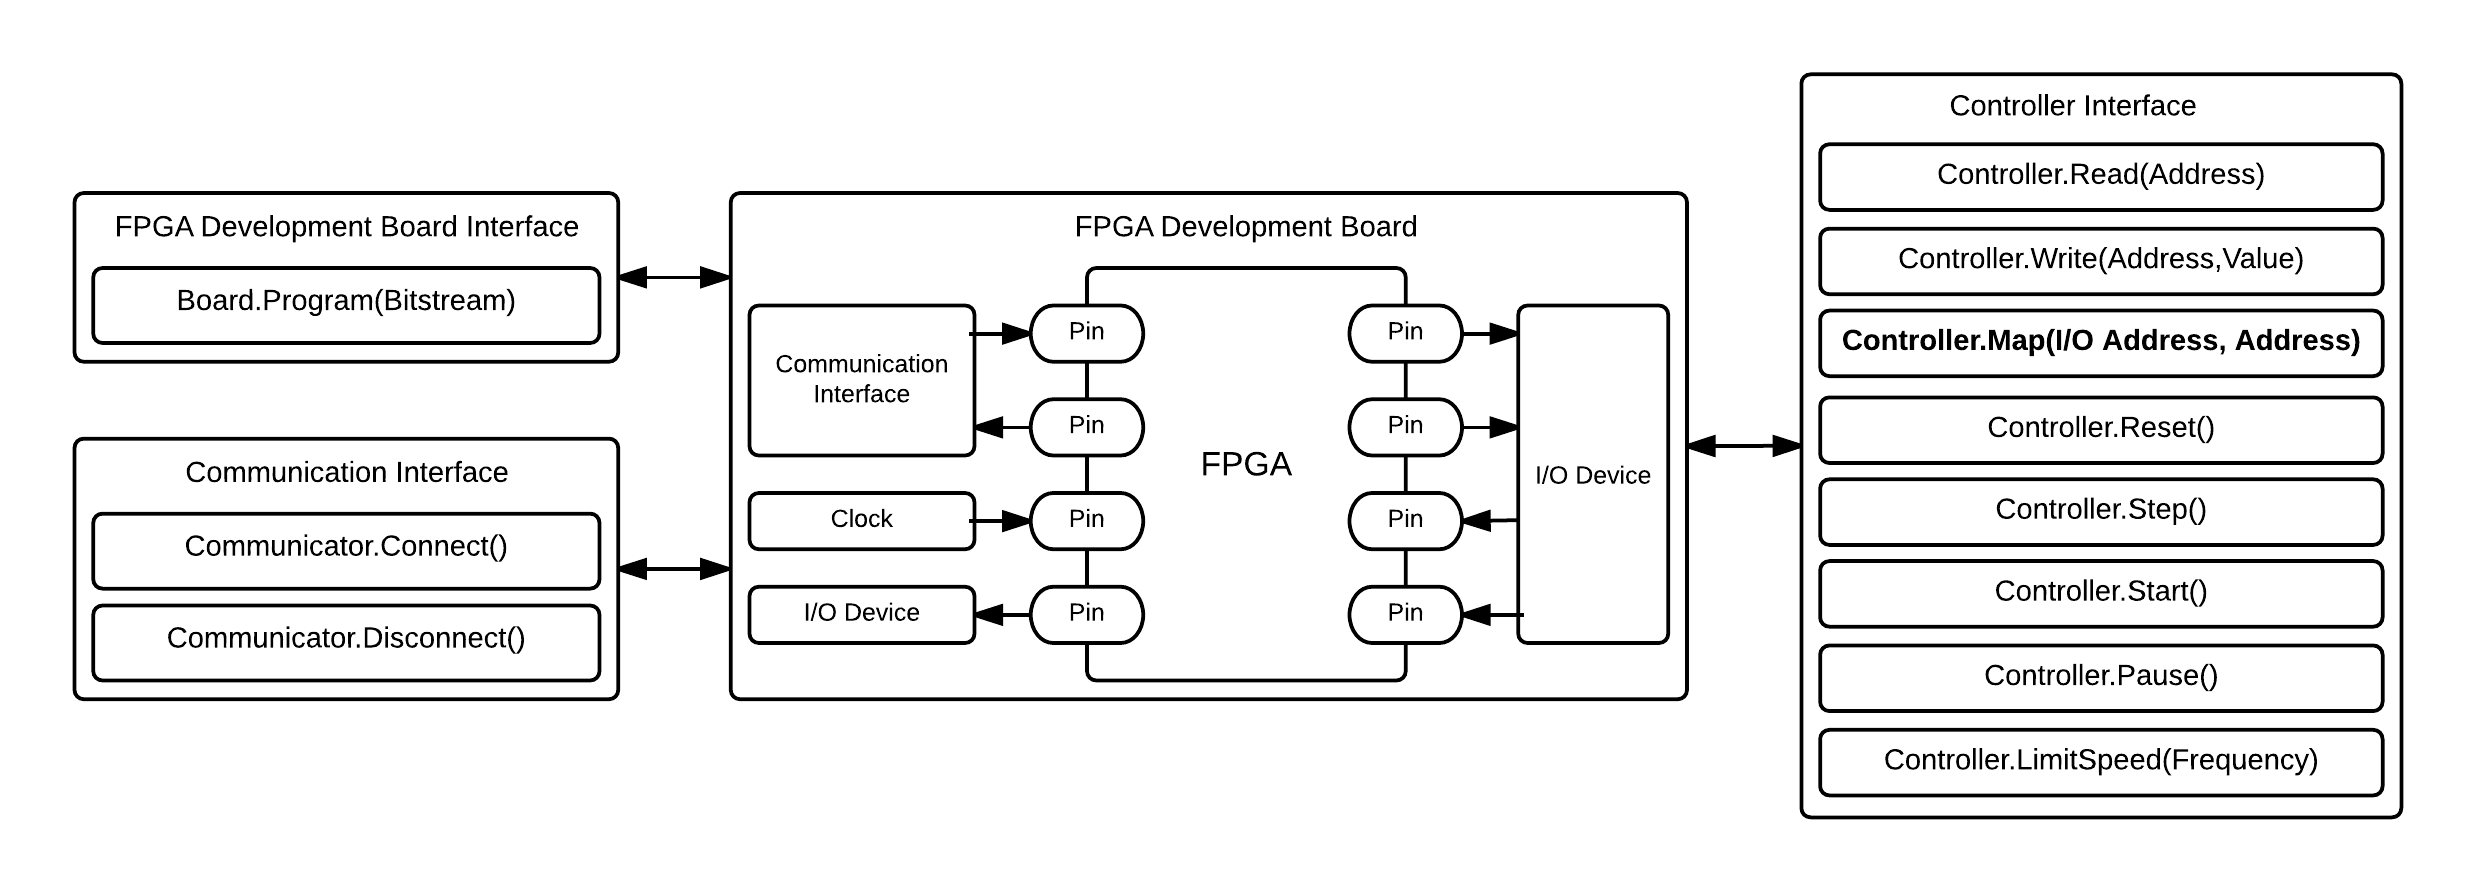
\includegraphics[width=\textwidth]{img/overview-io}
\caption{I/O reintroduced, overview}
\label{fig:overview-io}
\end{figure}


\begin{figure}[h]
\centering
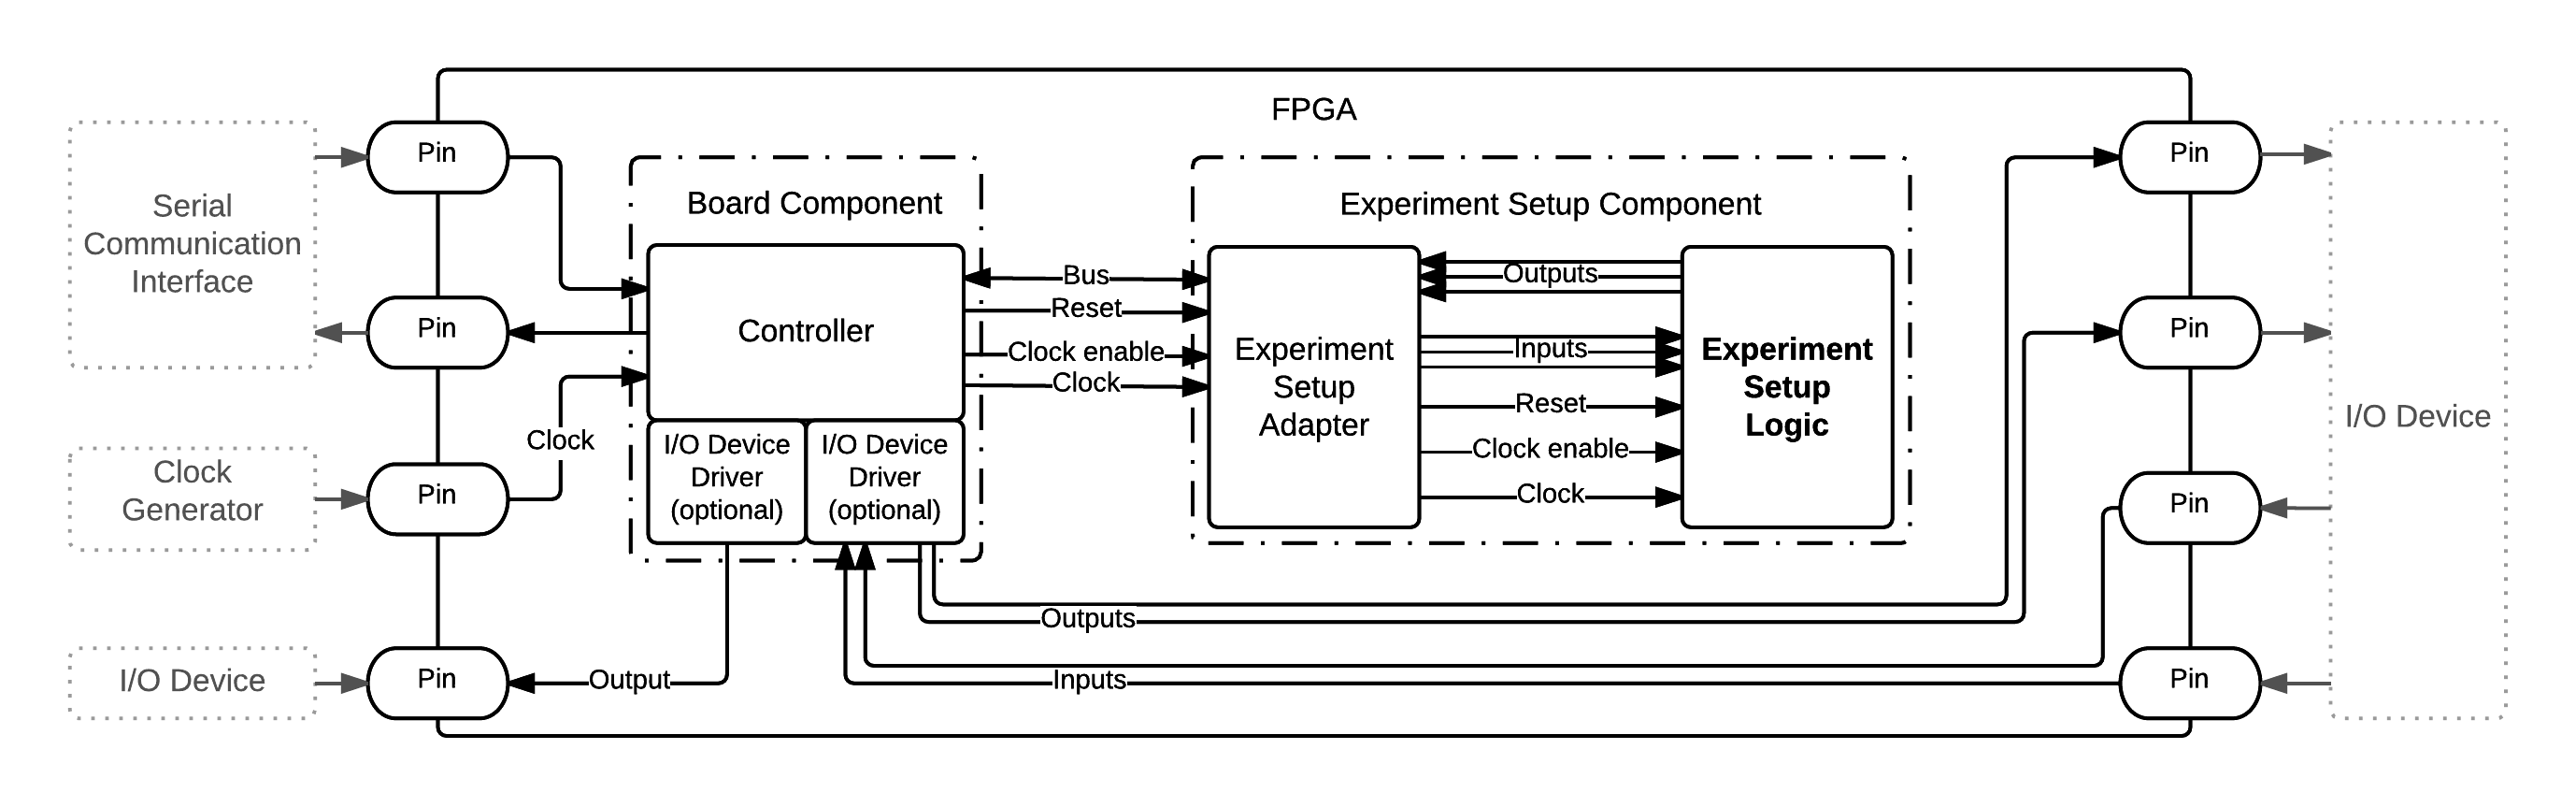
\includegraphics[width=\textwidth]{img/fpga-io2}
\caption{I/O reintroduced, FPGA logic design}
\label{fig:fpga-io}
\end{figure}

% \begin{figure}
% \centering
% \includegraphics[width=\textwidth]{processes-dependencies-io}
% \caption{I/O reintroduced, Process dependency graph}
% \label{fig:processes-dependencies}
% \end{figure}

% \begin{figure}
% \centering
% \makebox[\textwidth][c]{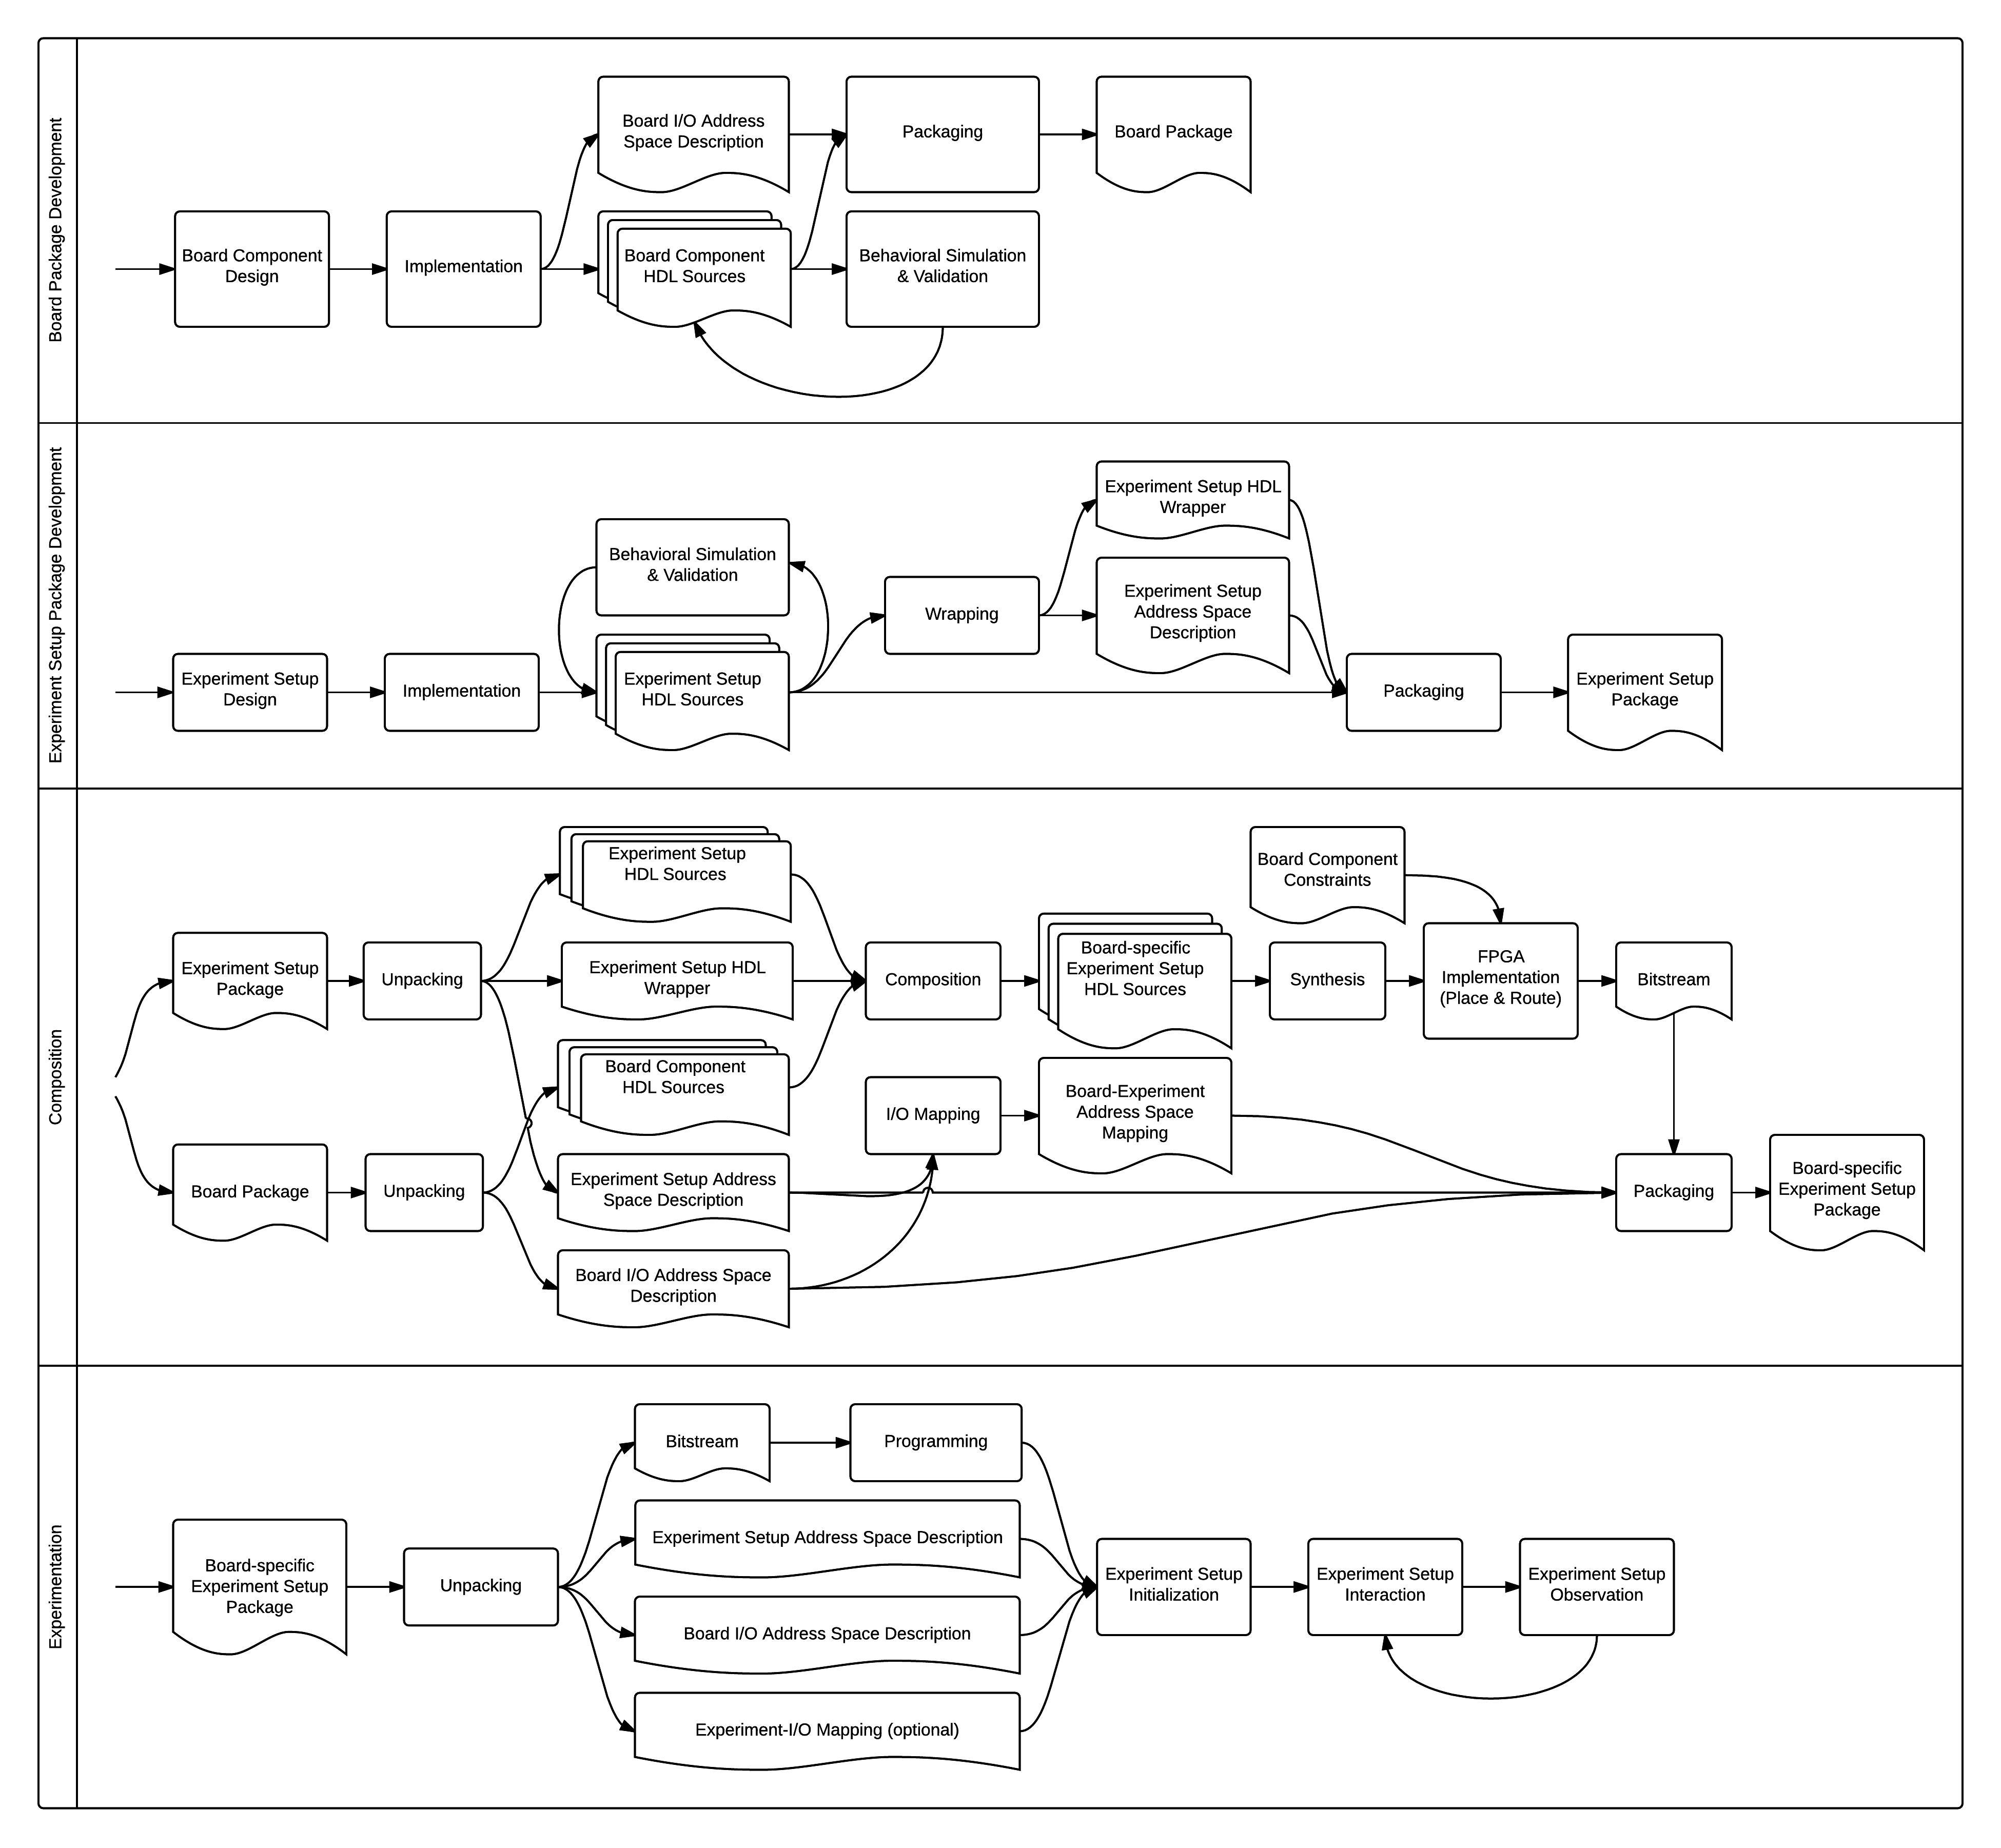
\includegraphics[width=1.25\textwidth]{processes-io}}
% \caption{I/O reintroduced, Processes overview}
% \label{fig:processes-io}
% \end{figure}

% \section{Student Requirements}
% A FPGA development board is connected to a student's PC. Two issues need to be addressed: an easy way of programming the FPGA in order to setup the experiment and communication with the FPGA to allow for interaction during the experiment. 

% Manufacturer development tools often facilitate these functions.

% They install FPGA board operating system drivers and experiment host software. An experiment is prepared by the course instructors and distributed to students. By loading the experiment, the fpga should be automatically programmed. The FPGA is not reprogrammed during the experiment. The student only interacts with the experiment through the experiment host software or the physical board as if it were the experiment hardware itself. 

% \section{Instructor requirements}
% It should be easy for instructors to create, test and distribute experiments. For the development of these experiments, instructors should be able to make use of existing development tools. 

% \section{Conceptual Model}
% In combinatorial logic, the output of signals is not dependent on the state of the digital circuit. In sequential logic, the output is dependent on the input signal levels, as well as the levels of previous input signals, the state of the circuit. Sequential logic is usually synchronous, meaning that state changes are triggered by a clock signal. 

% The circuit's state needs to be transfered to the student's PC such that it can be interpreted. 

% From an abstract point of view, a sequential circuit's state can be seen as a series of signals. Some signals are singular bit values, while others are composed of multiple bit values. Signals can be independent, while similar may be grouped by function, such as a set of cpu registers, data memory or instruction memory. 

% All these signals may be projected onto a memory space in order to allow for all signals of an experiment setup to be represented uniformly. 

% A file combined with the fpga program instructs the PC software on how to the memory space should be interpreted. This file is specific for one single version an FPGA program, but the same accross different FPGA board and desktop tools. In the fpga program it is determined how the experiment's signals are mapped onto the memory space. The PC software interprets these signals. 

% A fpga program may support multiple types of communication, such as serial rs232, ehternet, pci express etc...

% A distributable is specific for a combination of a FPGA development board model, a version of the FPGA program and a version of the PC tools. 

% The pc software must allow for the loading of a distributable, programming the experiment onto the FPGA and establishing a connection such that it can control the experiment. The PC software interprets the memory map of the fpga program and adapts its interface. After establishing a connection, the student can start the experiment by manually stepping a clock cycle, or set the clock cycle to increase automatically at a defined frequency. 

\chapter{Implementation}
In order to test the proposed framework, an implementation is provided. The framework implementation is targeted at the Digilent Nexys 4 FPGA development board, displayed in figure \ref{fig:nexys4}. This board contains a Xilinx Artix-7 series FPGA and is equipped with various I/O devices. The development board is connected with the PC through USB. This USB connection is used in order to setup a serial communication channel between the PC and the FPGA.

\begin{itemize}
\item PC Software Interface Standardization
\item PC Software Development
\item FPGA Development Board PC Software Plugin Development
\begin{itemize}
\item For a specific FPGA Development Board PC Driver
\end{itemize}
\item Board Package Interface Standardization
\item Board Package Development
\begin{itemize}
\item For a specific FPGA Development Board
\end{itemize}
\item Experiment Wrapping Toolchain Development
\item Composition Toolchain Development
\begin{itemize}
\item For a specific FPGA Compilation Toolchain
\end{itemize}
\item Experiment Setup Development
\end{itemize}


\section{Functional}
Reset button behaviour.

\begin{figure}
\centering
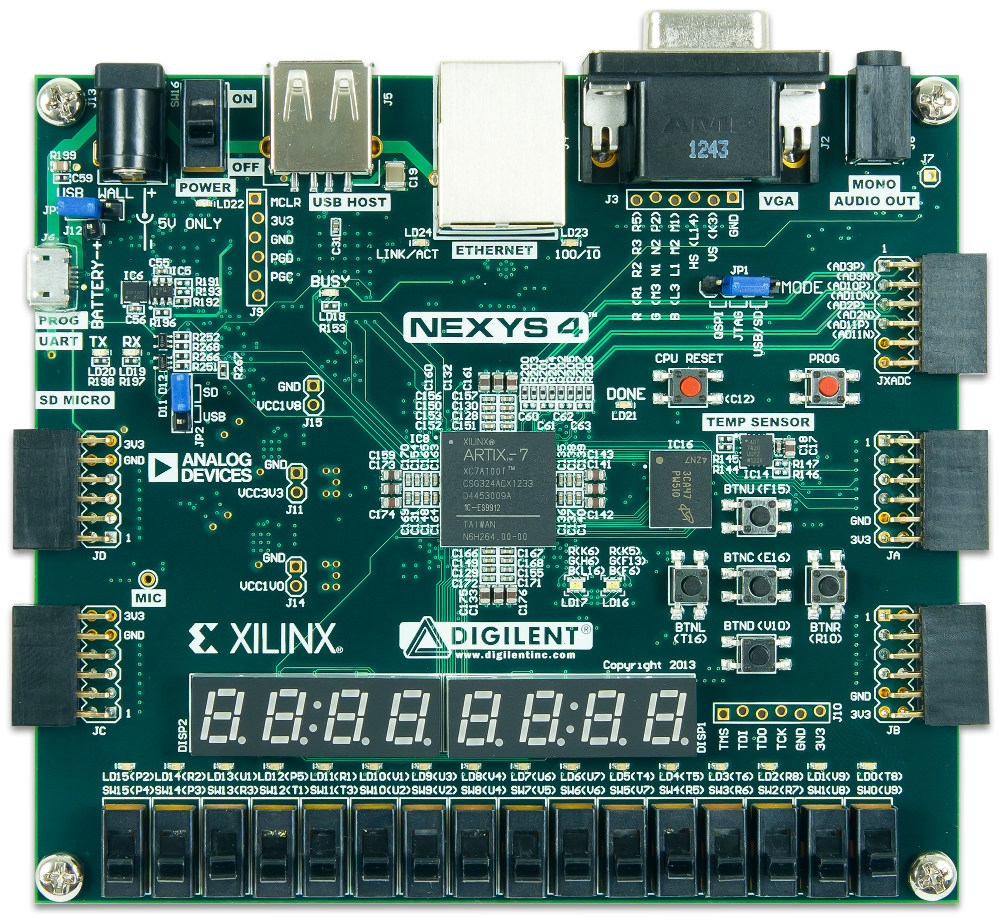
\includegraphics[width=0.7\textwidth]{img/nexys4-small}
\caption{Digilent Nexys 4 Artix-7 FPGA development board}
\label{fig:nexys4}
\end{figure}

\chapter{Experimental results}

\appendix

\chapter{Process Analysis}

\begin{figure}[h]
\centering
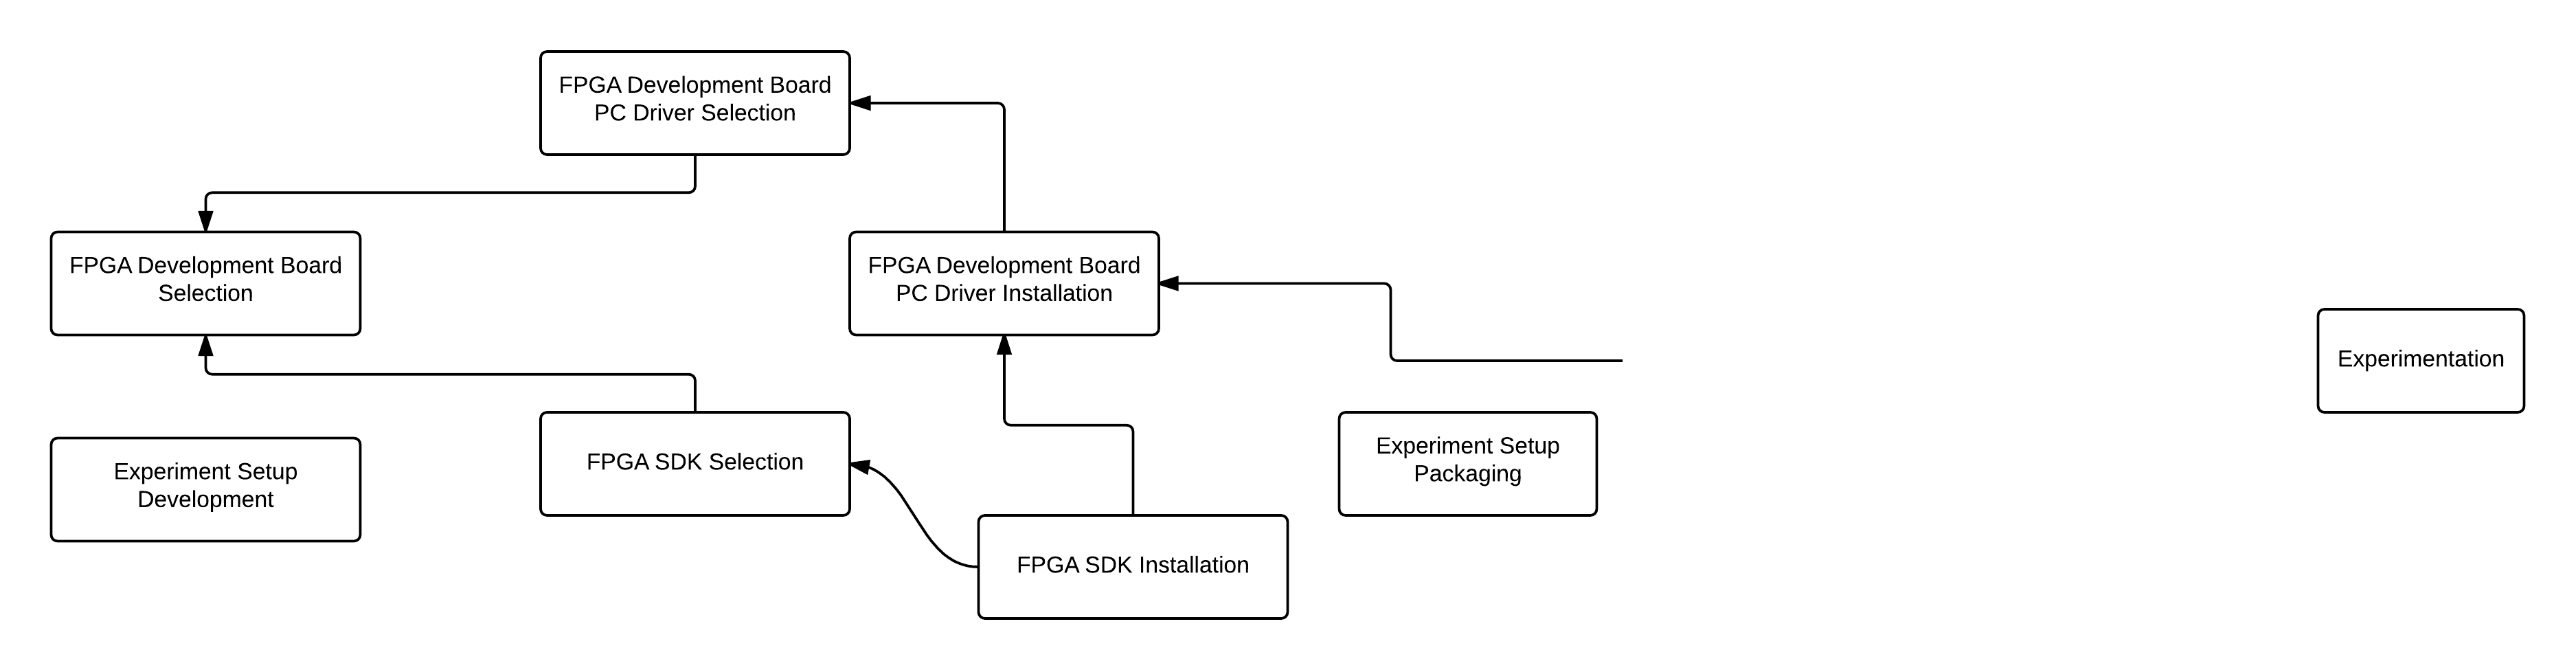
\includegraphics[width=\textwidth]{img/processes-dependencies-basic}
\caption{The basic model, process dependency graph}
\label{fig:dependencies-basic}
\end{figure}

\begin{figure}[h]
\centering
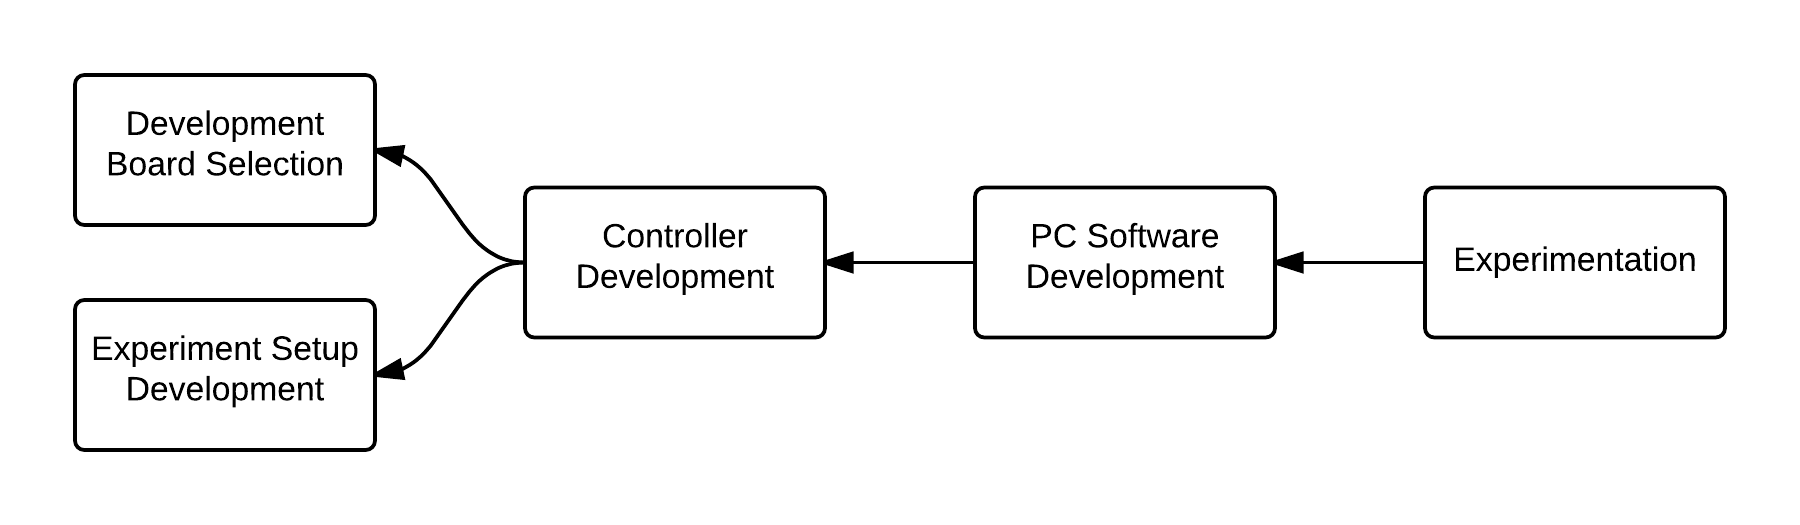
\includegraphics[width=\textwidth]{img/processes-dependencies-inout}
\caption{I/O virtualized, process dependency graph}
\label{fig:dependencies-inout}
\end{figure}

\begin{landscape}
\begin{figure}
\centering
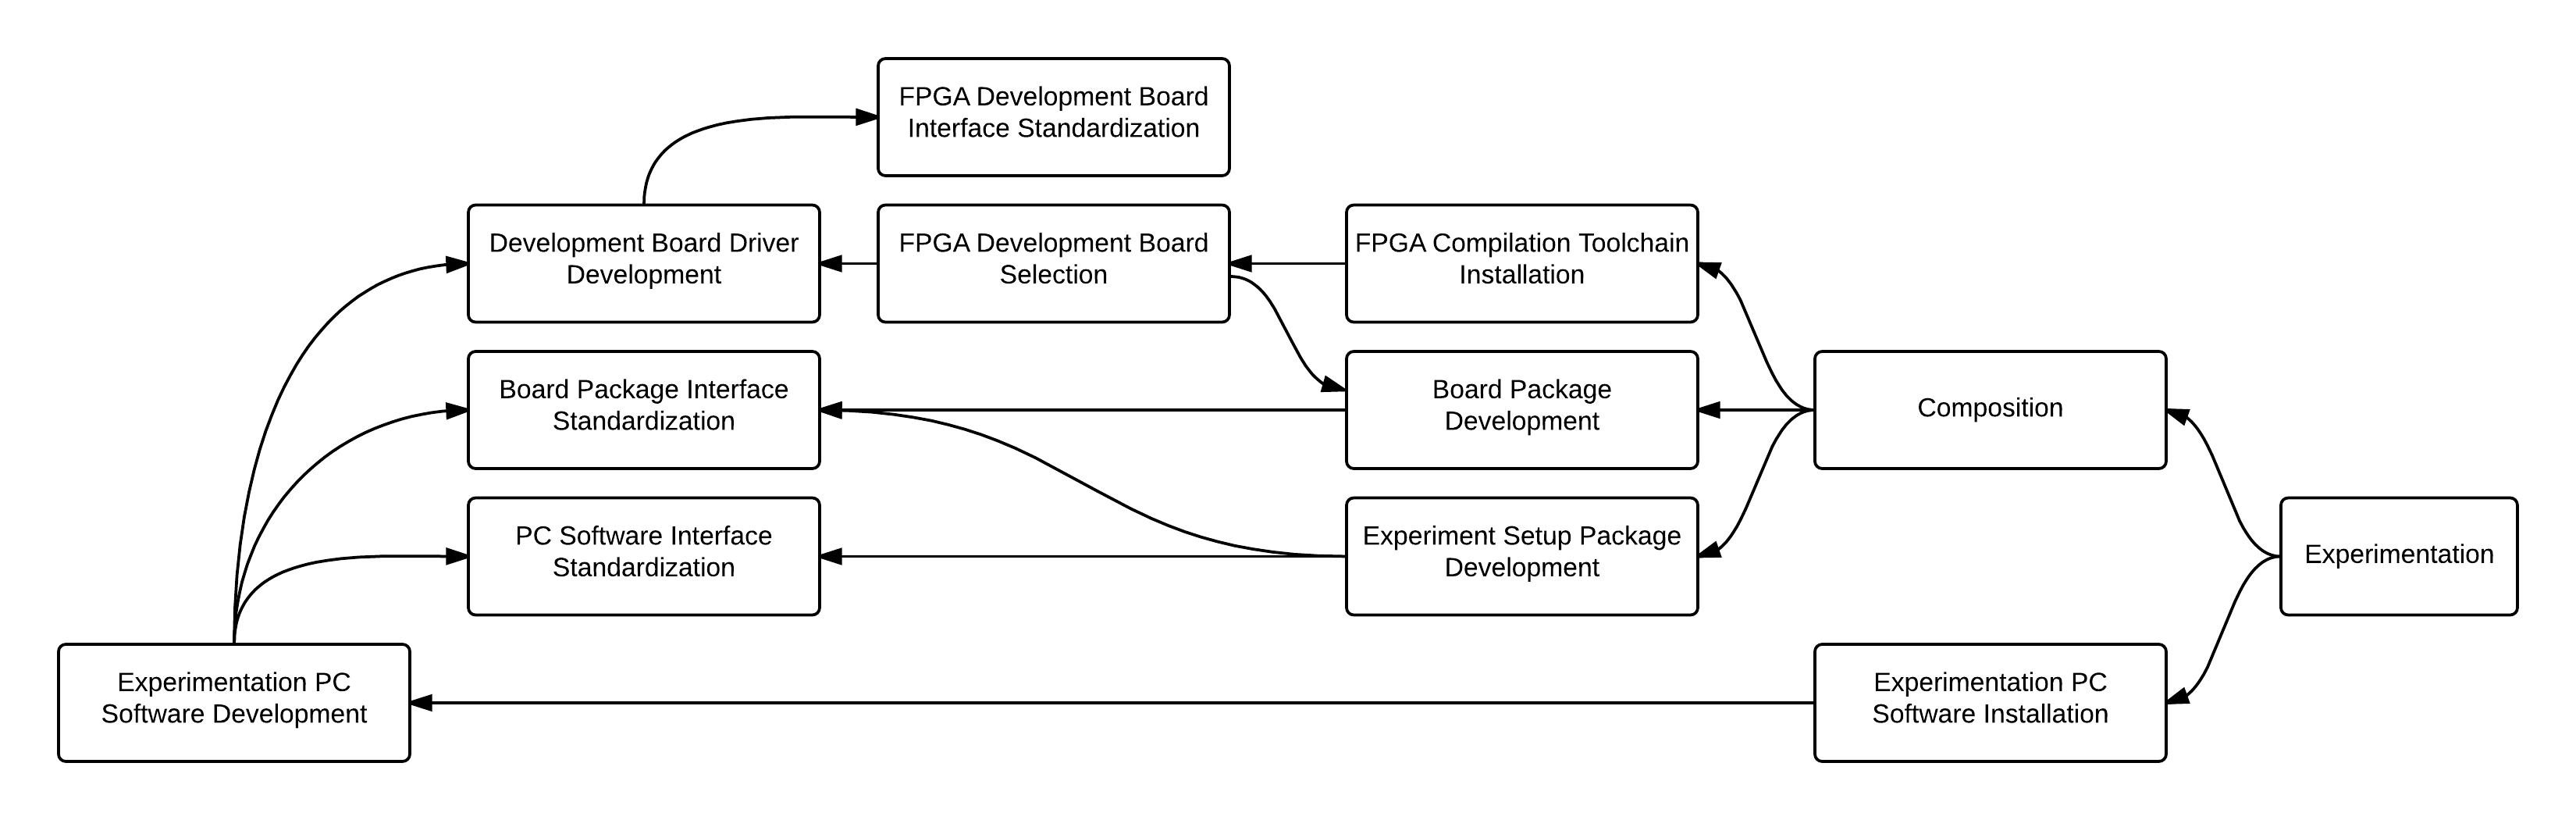
\includegraphics[width=\hsize]{img/processes-dependencies-control}
\caption{Cycle control, process dependency graph}
\label{fig:dependencies-control}
\end{figure}
\end{landscape}

\begin{landscape}
\begin{figure}
\centering
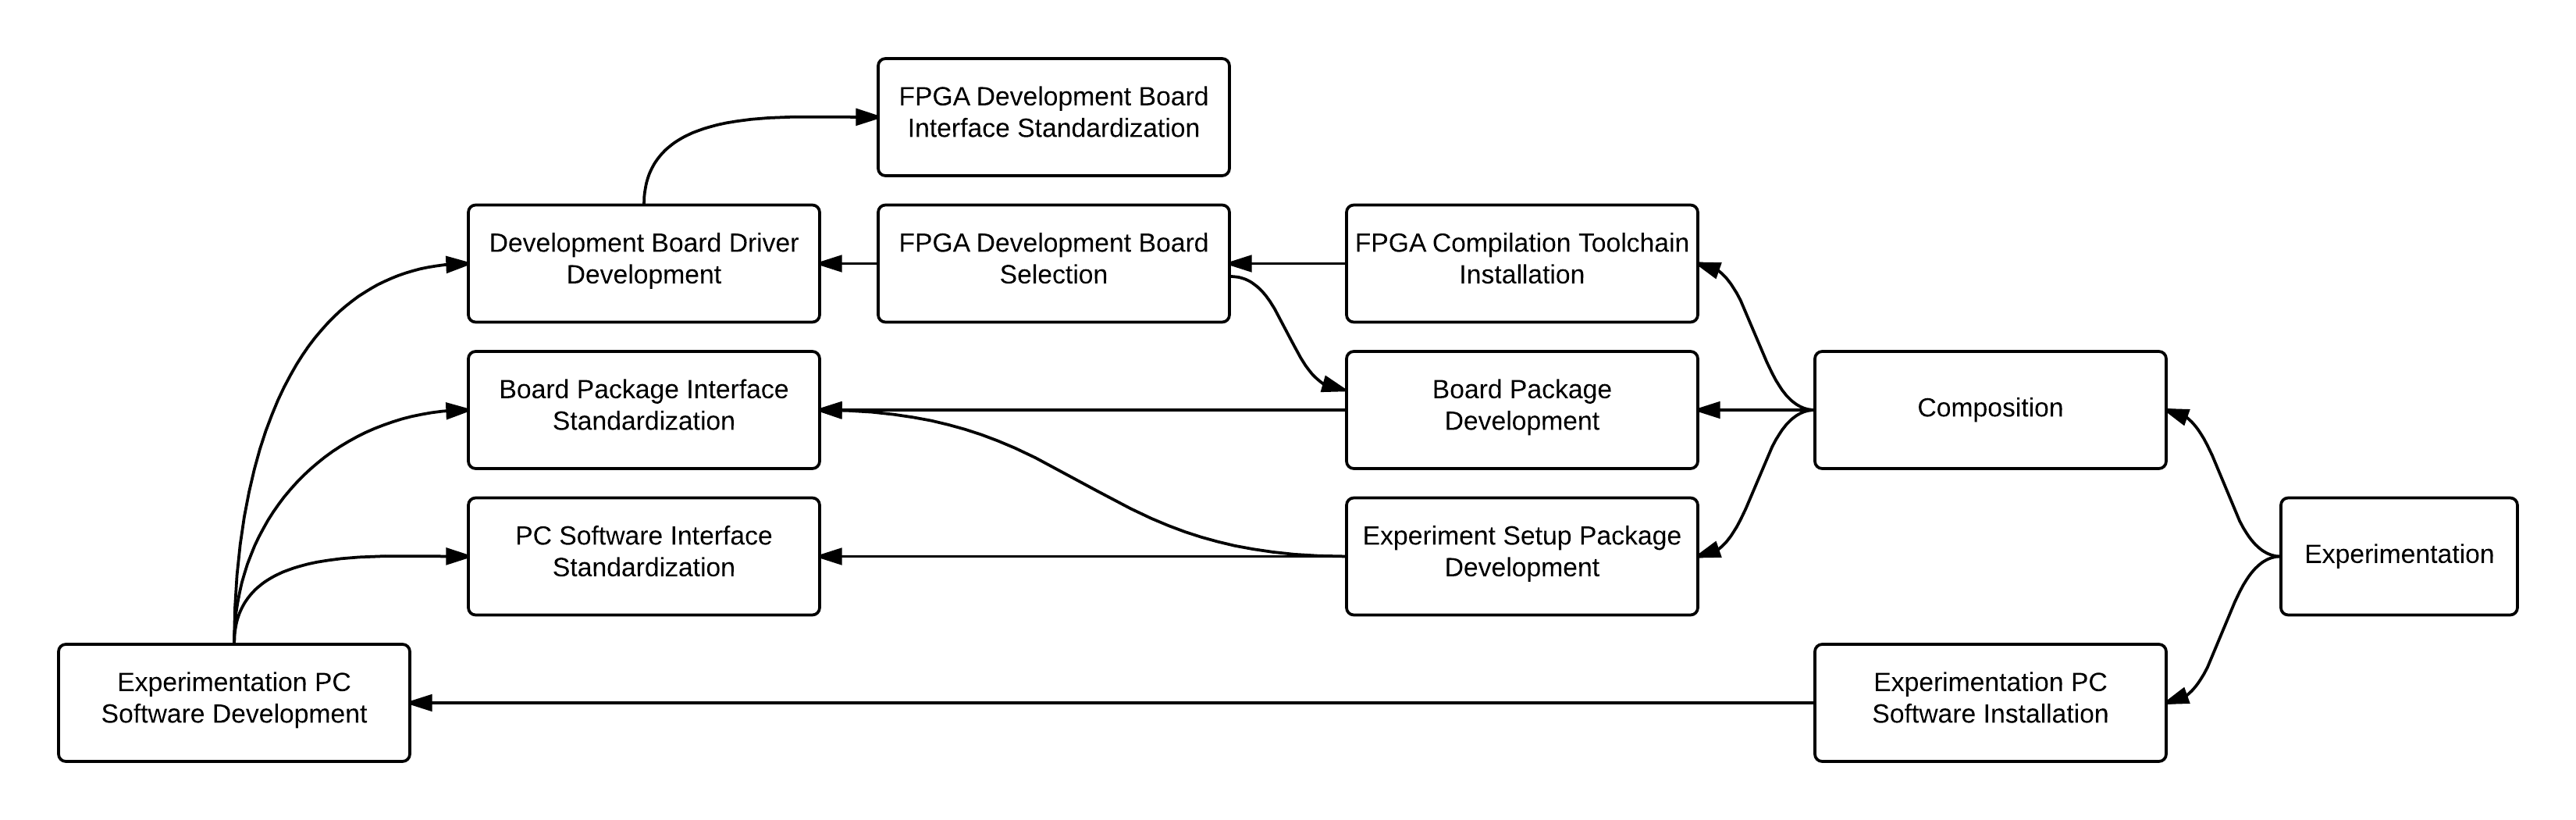
\includegraphics[width=\hsize]{img/processes-dependencies-abstract}
\caption{Controller abstracted, process dependency graph}
\label{fig:dependencies-abstract}
\end{figure}
\end{landscape}

\begin{landscape}
\begin{figure}
\centering
\includegraphics[width=\hsize]{img/processes-dependencies-io}
\caption{I/O reintroduced, process dependency graph}
\label{fig:dependencies-io}
\end{figure}
\end{landscape}





\chapter{Logic Diagrams}

\section{Simple wrapping}
\begin{figure}[h]
    \centering
    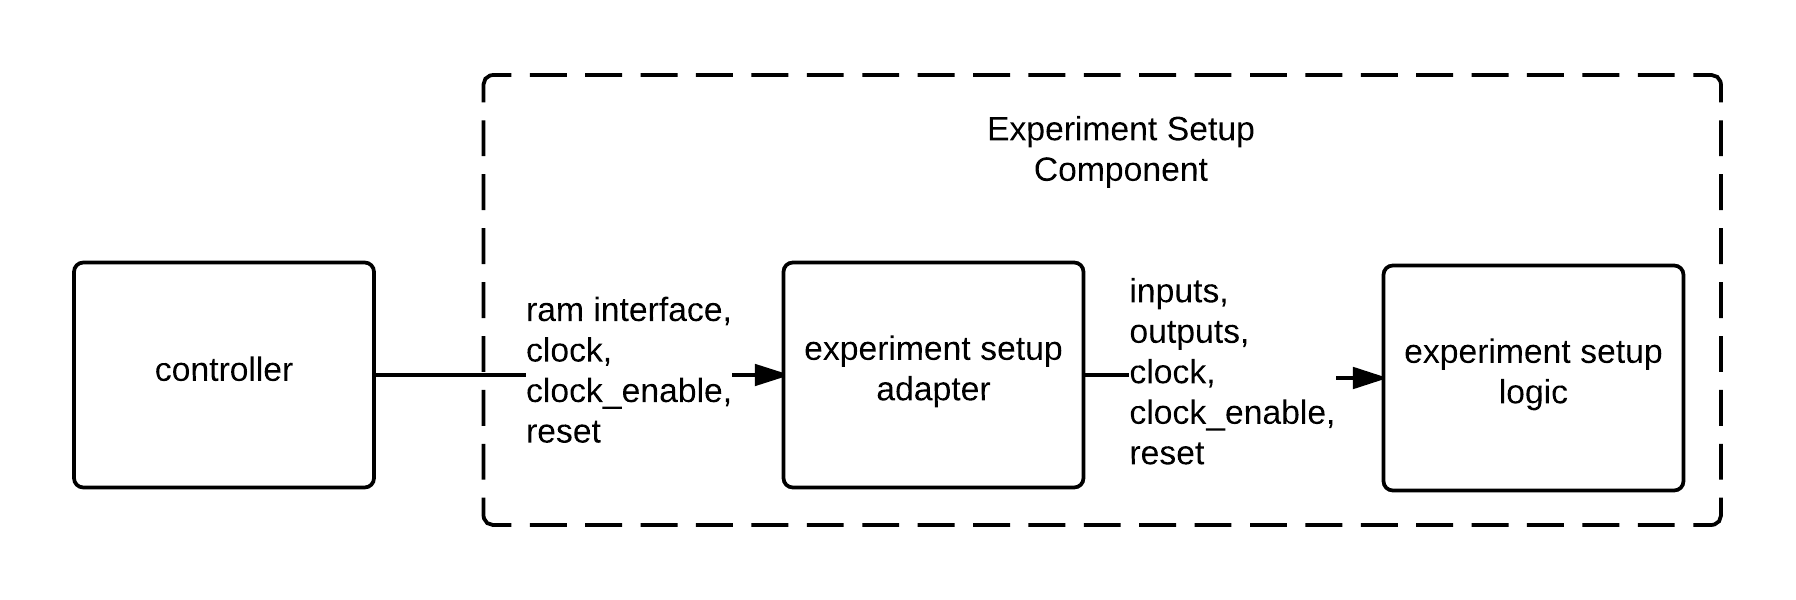
\includegraphics[width=\textwidth]{img/logic-wrap-simple}
    \caption{Caption}
    \label{fig:logic-wrap-simple}
\end{figure}

\begin{landscape}
    \section{Advanced wrapping}
    \begin{figure}[h]
        \centering
        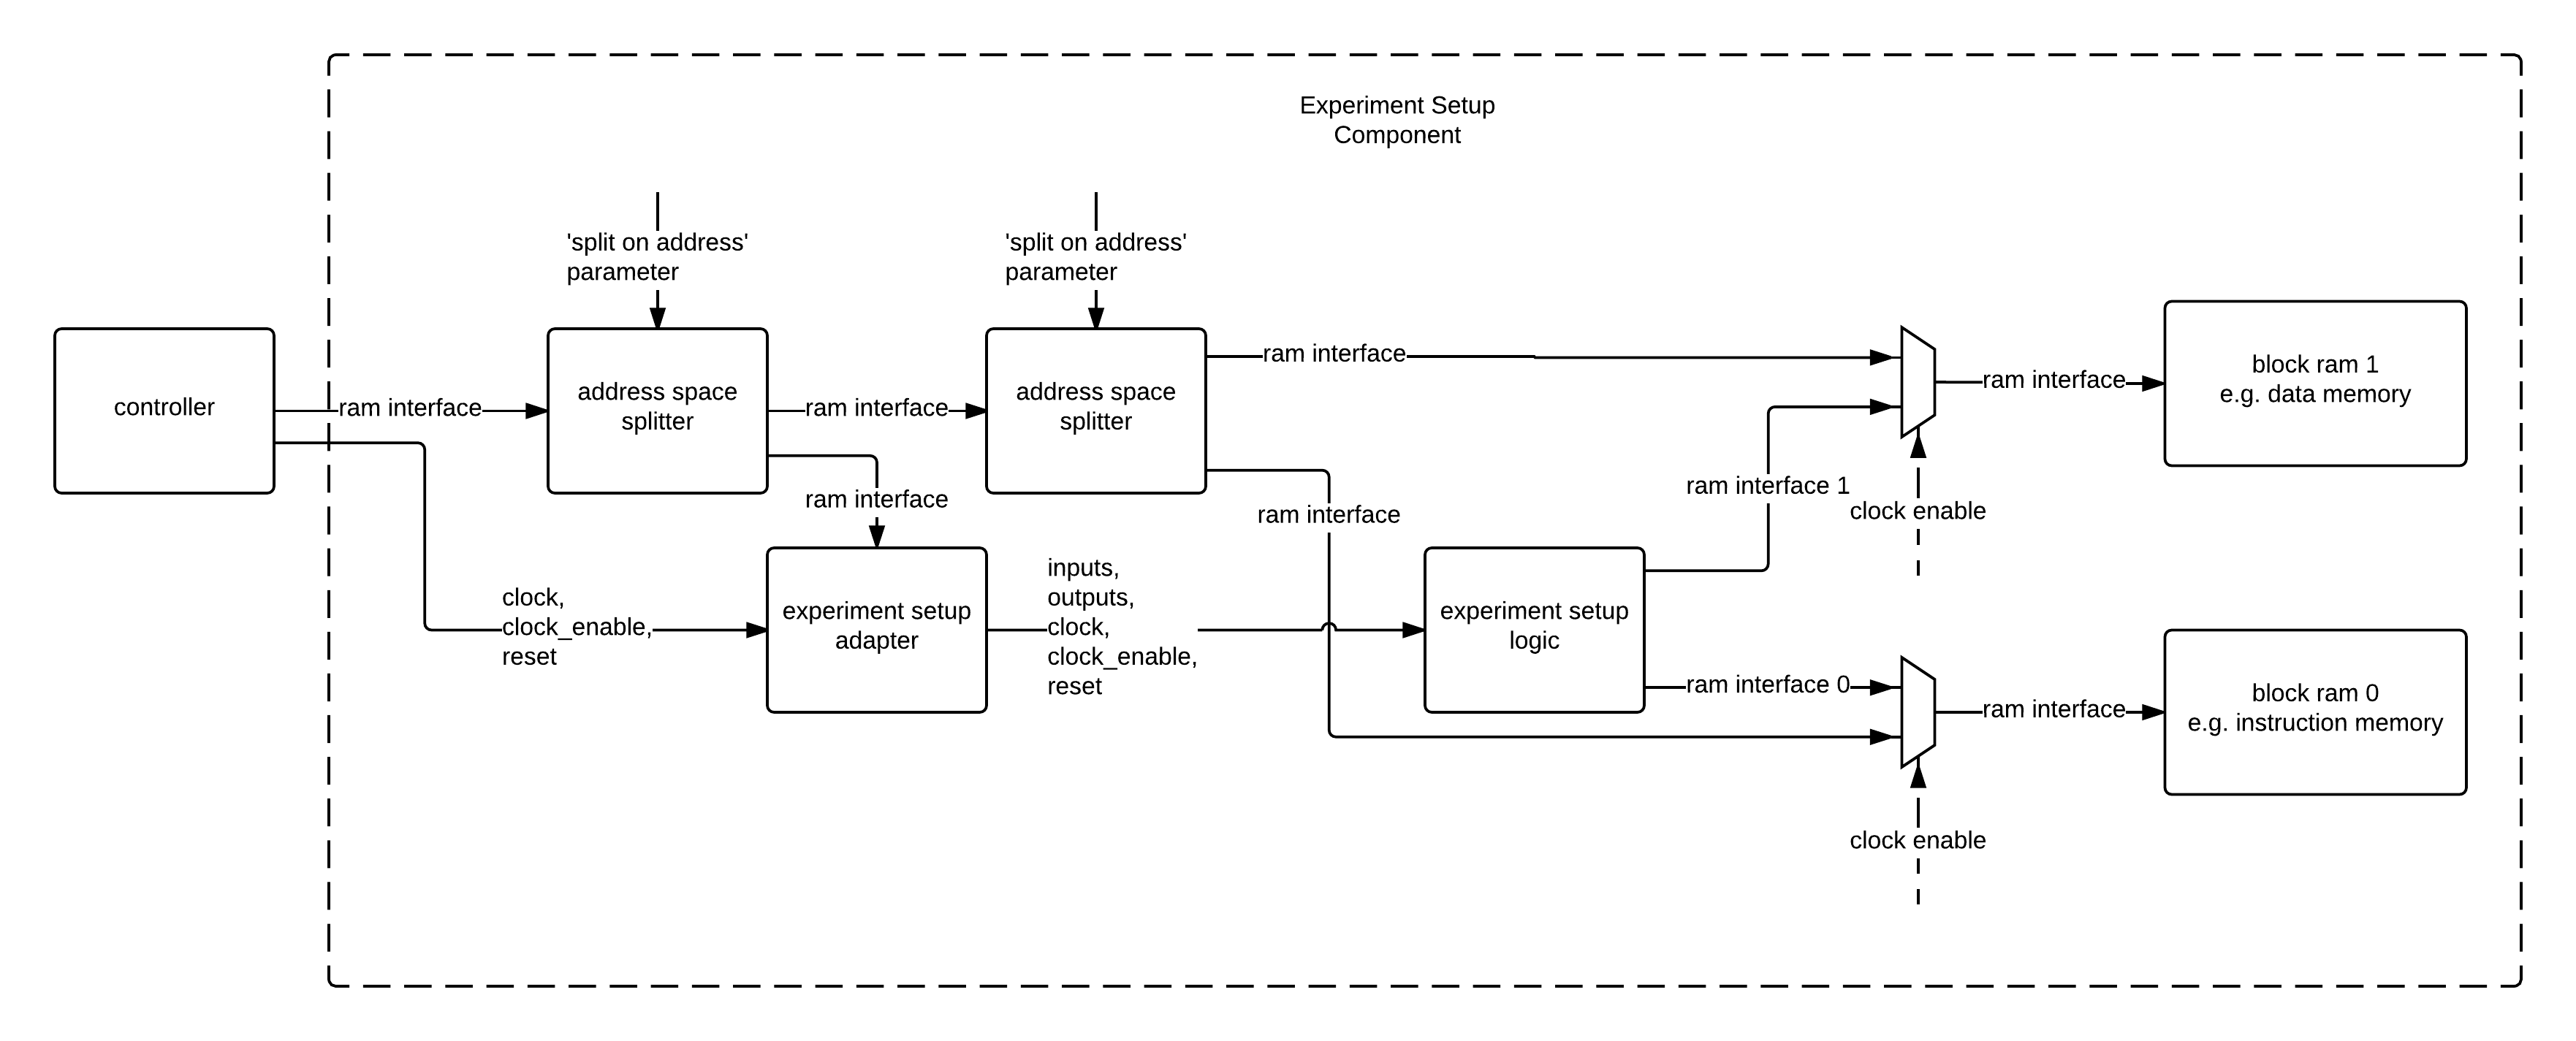
\includegraphics[width=\hsize]{img/logic-wrap-extended}
        \caption{Complex wrapper}
        \label{fig:logic-wrap-extended}
    \end{figure}
\end{landscape}

\section{Experiment Adapter}
\begin{figure}[h]
    \centering
    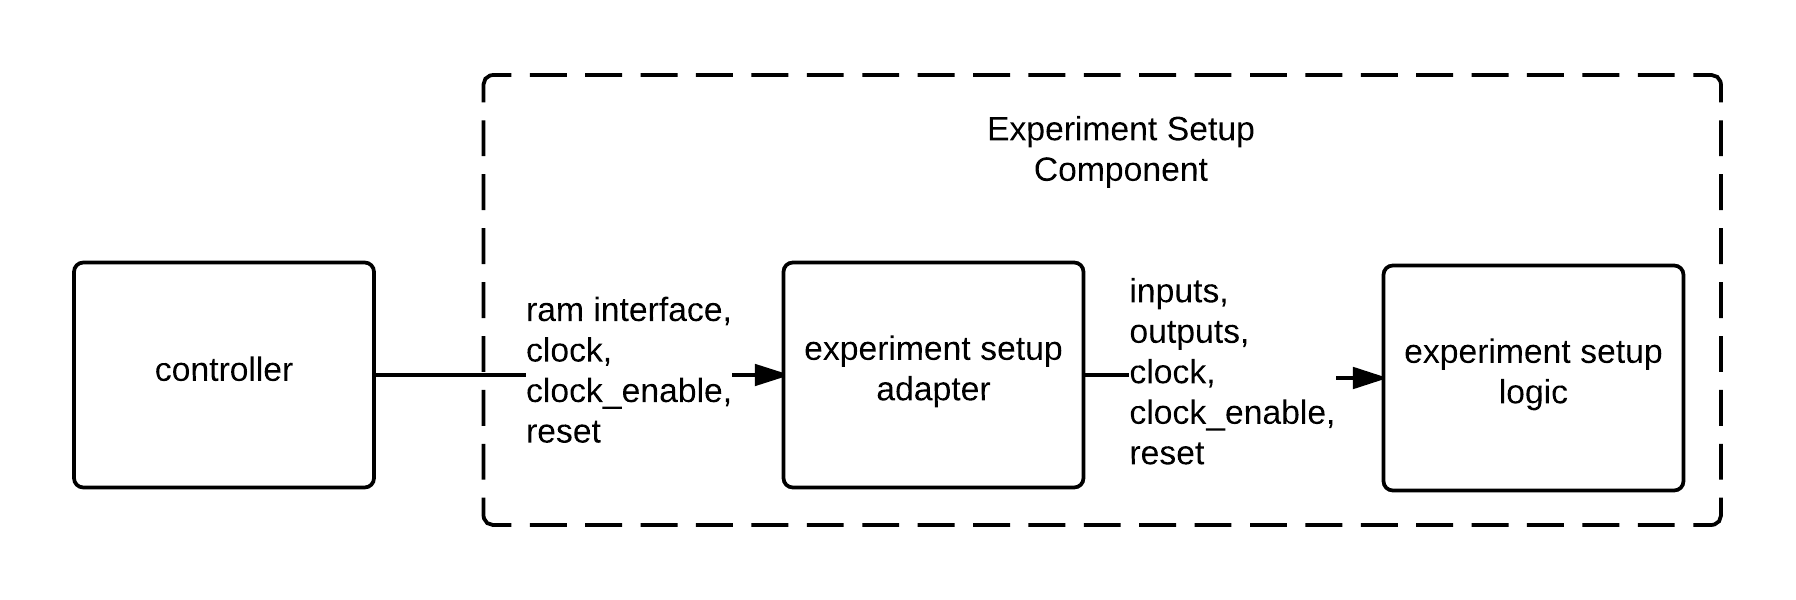
\includegraphics[width=\textwidth]{img/logic-wrap-simple}
    \caption{Caption}
    \label{fig:logic-experiment-adapter}
\end{figure}

\cleardoublepage

\addcontentsline{toc}{chapter}{Bibliography}
\phantomsection

\printbibliography

\end{document}